%%%%%%%%%%%%%%%%%%%%%%%%%%%%%%%%%%%%%%%%%%%%%%%%%%%%%%%%%%%%%%%%%%%%%%%%%%%%%%%
%
% REPORT  DESCRIPTION:
%   A concise description of the main concepts of the capstone.
%
% RESEARCH:
%   A list of research activities which led to this capstone.
%
% EXPERIMENTS:
%   A list of the experiments performed which supported the research.
%
%%%%%%%%%%%%%%%%%%%%%%%%%%%%%%%%%%%%%%%%%%%%%%%%%%%%%%%%%%%%%%%%%%%%%%%%%%%%%%%
\documentclass[12pt,american]{report}
\usepackage{rit-cs-capstone}
%%%%%%%%%%%%%%%%%%%%%%%%%%%%%%%%%%%%%%%%%%%%%%%%%%%%%%%%%%%%%%%%%%%%%%%%%%%%%%%
%   The following packages are all optional and depend on the specifics of what
% is contained in the capstone.  There is no harm in leaving them in.
%%%%%%%%%%%%%%%%%%%%%%%%%%%%%%%%%%%%%%%%%%%%%%%%%%%%%%%%%%%%%%%%%%%%%%%%%%%%%%%
\usepackage{subfigure}
\usepackage[refpages]{gloss}
\usepackage{babel}
\usepackage{times}
\usepackage{graphicx}
\usepackage{amssymb}
\usepackage{lscape}
\usepackage{verbatim}
\usepackage{enumerate}
\usepackage{afterpage}
\usepackage{url}
\usepackage{amsmath}
\usepackage[chapter]{algorithm}
\usepackage{algpseudocode}
\usepackage{hyperref}
%%%%%%%%%%%%%%%%%%%%%%%%%%%%%%%%%%%%%%%%%%%%%%%%%%%%%%%%%%%%%%%%%%%%%%%%%%%%%%%
%   Mark the document as 'draft' with a date. Be sure to comment this out for
% the final version.
%\usepackage{watermark}
%\watermark{\hspace{-0.3in} \textbf{DRAFT} \hspace{2.0in} \textbf{\today}}
%%%%%%%%%%%%%%%%%%%%%%%%%%%%%%%%%%%%%%%%%%%%%%%%%%%%%%%%%%%%%%%%%%%%%%%%%%%%%%%

\makegloss

\begin{document}
%%%%%%%%%%%%%%%%%%%%%%%%%%%%%%%%%%%%%%%%%%%%%%%%%%%%%%%%%%%%%%%%%%%%%%%%%%%%%%%
% Title page
% The \title{} can contain line breaks as appropriate...
\title{\vspace{-0.20in} Evaluation of Hill Climbing attack method\\
   on SHA-3 Finalist}
% The \titleline{} must have no line breaks in it.
\titleline{MS Project Proposal}
% This is not a thesis but a project
\MSprojecttrue
% This date is really not used (unless \grantdate{}{} is blank)
\date{July 2013}
%%%%%%%%%%%%%%%%%%%%%%%%%%%%%%%%%%%%%%%%%%%%%%%%%%%%%%%%%%%%%%%%%%%%%%%%%%%%%%%

%%%%%%%%%%%%%%%%%%%%%%%%%%%%%%%%%%%%%%%%%%%%%%%%%%%%%%%%%%%%%%%%%%%%%%%%%%%%%%%
% Author information page
% The \author{} should be exactly the same as your diploma
\author{Soham Sadhu}
%%%%%%%%%%%%%%%%%%%%%%%%%%%%%%%%%%%%%%%%%%%%%%%%%%%%%%%%%%%%%%%%%%%%%%%%%%%%%%%

%%%%%%%%%%%%%%%%%%%%%%%%%%%%%%%%%%%%%%%%%%%%%%%%%%%%%%%%%%%%%%%%%%%%%%%%%%%%%%%
% The following information is for the signature page.
% Note that the definition for principal adviser uses two fields.
% This was needed so that the adviser's name could be placed on the
% abstract page without his/her title.
\committeechair{Dr. Stanis{\l}aw Radziszowski}{Professor}
%\reader{Alan Kaminsky \\ Professor}
%\observer{Dr. Edith Hemaspaandra \\ Professor}
%%%%%%%%%%%%%%%%%%%%%%%%%%%%%%%%%%%%%%%%%%%%%%%%%%%%%%%%%%%%%%%%%%%%%%%%%%%%%%%

%%%%%%%%%%%%%%%%%%%%%%%%%%%%%%%%%%%%%%%%%%%%%%%%%%%%%%%%%%%%%%%%%%%%%%%%%%%%%%%
% This is the expected date that the committee will sign your Capstone.
\grantdate{July}{2013}
%%%%%%%%%%%%%%%%%%%%%%%%%%%%%%%%%%%%%%%%%%%%%%%%%%%%%%%%%%%%%%%%%%%%%%%%%%%%%%%

%%%%%%%%%%%%%%%%%%%%%%%%%%%%%%%%%%%%%%%%%%%%%%%%%%%%%%%%%%%%%%%%%%%%%%%%%%%%%%%
% If you want to copyright your capstone remove the line below.
\copyrightfalse% True by default
% The year of the copyright; usually same as the date the committee will
% sign the \item{} . This won't be printed if \copyrightfalse
\copyrightyear{2013}
%%%%%%%%%%%%%%%%%%%%%%%%%%%%%%%%%%%%%%%%%%%%%%%%%%%%%%%%%%%%%%%%%%%%%%%%%%%%%%%

%%%%%%%%%%%%%%%%%%%%%%%%%%%%%%%%%%%%%%%%%%%%%%%%%%%%%%%%%%%%%%%%%%%%%%%%%%%%%%%
% This causes all front matter to be set.
\beforepreface%
%%%%%%%%%%%%%%%%%%%%%%%%%%%%%%%%%%%%%%%%%%%%%%%%%%%%%%%%%%%%%%%%%%%%%%%%%%%%%%%

%%%%%%%%%%%%%%%%%%%%%%%%%%%%%%%%%%%%%%%%%%%%%%%%%%%%%%%%%%%%%%%%%%%%%%%%%%%%%%%
% The dedication - if you choose to include one.
% It should be vertically centered in the page. Since the style format doesn't 
% do it for you automatically, you can use the following technique.
%\prefacesection{Dedication}
%\vfill
%\begin{center}
%To my parents.
%\end{center}
%\vfill
%%%%%%%%%%%%%%%%%%%%%%%%%%%%%%%%%%%%%%%%%%%%%%%%%%%%%%%%%%%%%%%%%%%%%%%%%%%%%%%

%%%%%%%%%%%%%%%%%%%%%%%%%%%%%%%%%%%%%%%%%%%%%%%%%%%%%%%%%%%%%%%%%%%%%%%%%%%%%%%
% The acknowledgements page - if you choose to include one. 
% As in the dedication, it should be centered vertically in the page.
%
%\prefacesection{Acknowledgments}
%\vfill
%\begin{center}
%\indent I am grateful to Prof. Stanis{\l}aw Radziszowski, for his guidance.
%\end{center}
%\vfill
%%%%%%%%%%%%%%%%%%%%%%%%%%%%%%%%%%%%%%%%%%%%%%%%%%%%%%%%%%%%%%%%%%%%%%%%%%%%%%%

%%%%%%%%%%%%%%%%%%%%%%%%%%%%%%%%%%%%%%%%%%%%%%%%%%%%%%%%%%%%%%%%%%%%%%%%%%%%%%%
%%  Collection of useful abbreviations.
\newcommand{\etc} {\emph{etc.\/}}
\newcommand{\etal}{\emph{et~al.\/}}
\newcommand{\eg}  {\emph{e.g.\/}}
\newcommand{\ie}  {\emph{i.e.\/}}
%%%%%%%%%%%%%%%%%%%%%%%%%%%%%%%%%%%%%%%%%%%%%%%%%%%%%%%%%%%%%%%%%%%%%%%%%%%%%%%


%%%%%%%%%%%%%%%%%%%%%%%%%%%%%%%%%%%%%%%%%%%%%%%%%%%%%%%%%%%%%%%%%%%%%%%%%%%%%%%
% Abstract
\begin{abstractpage}

Digital signatures applied in \href{"http://en.wikipedia.org/wiki/Cryptographic\_hash\_function\#Applications"}
{computer security}, are created and verified using cryptographic hash functions \cite{00042}.
The \href{"http://www.nist.gov/index.html"}{National Institute of Standards and Technology (NIST)} has published
family of cryptographic hash algorithms known as \href{http://en.wikipedia.org/wiki/Secure_Hash_Algorithm}
{Secure Hash Algorithm (SHA)} as U.S \href{http://en.wikipedia.org/wiki/Federal_Information_Processing_Standard}
{Federal Information Processing Standards (FIPS)}.

Due to advances in cryptanalysis of SHA-2, NIST announced a competition in November, 2007 to choose SHA-3. 
All the 64 submissions to NIST were open to public for cryptanalysis. 
In October, 2012 \href{"http://keccak.noekeon.org/"}{Keccak} was announced as the winner of SHA-3 competition. 
\href{"http://csrc.nist.gov/groups/ST/hash/sha-3/sha-3\_selection\_announcement.pdf"}{Keccak was chosen}
for its robustness and high security margin.

Of the 64 submissions for SHA-3 competition, 56 were selected for the first round, and 5 made it final round.
In this project I have compared the resistance to near collisions, on reduced versions of Keccak and two other
finalist \href{"https://131002.net/blake/"}{BLAKE}, and \href{"http://www.groestl.info/"}{Gr{\o}stl}. 
A $\epsilon / n $ bit near collision for hash function $h$ and two messages $M_{1}$ and $M_{2}$, where
$M_{1} \neq M_{2}$ is defined as
\begin{center}$HW( h( M_{1}, CV ) \oplus h( M_{2}, CV ) ) = n - \epsilon $\end{center}
where $HW$ is the Hamming weight, $h$ is the hash function, and $CV$ is the chaining value, and $n$ is the hash 
size in bits. I have also compared the near collision resistance amongst the different versions of Keccak by 
reducing its internal state size.

Hill climbing, simulated annealing, tabu search and random selection are applied to find a neighbourhood of chaining
value that is appended to two messages that are dissimilar by a bit, to find near collisions in the reduced versions 
of mentioned hashing algorithms.

Reduction in number of rounds predictably did reduce the security of hash function, but not by a large margin.
On other hand there was a inverse relation in increase in security margin and reduction in internal state size
of Keccak, for reduced rounds.
  
\end{abstractpage}

%%%%%%%%%%%%%%%%%%%%%%%%%%%%%%%%%%%%%%%%%%%%%%%%%%%%%%%%%%%%%%%%%%%%%%%%%%%%%%%

%%%%%%%%%%%%%%%%%%%%%%%%%%%%%%%%%%%%%%%%%%%%%%%%%%%%%%%%%%%%%%%%%%%%%%%%%%%%%%%
% Uncomment the line below if you don't want a list of tables to be printed.
% \tablespagefalse

% Uncomment the line below if you don't want a list of figures to be printed.
% \figurespagefalse

% \afterpreface generates the table of contents, list of tables (optional),
% and list of figures (optional).
\afterpreface%
\listofalgorithms
%%%%%%%%%%%%%%%%%%%%%%%%%%%%%%%%%%%%%%%%%%%%%%%%%%%%%%%%%%%%%%%%%%%%%%%%%%%%%%%

%We don't need a glossary so comment it out.
%\printgloss{Glossary}

%%%%%%%%%%%%%%%%%%%%%%%%%%%%%%%%%%%%%%%%%%%%%%%%%%%%%%%%%%%%%%%%%%%%%%%%%%%%%%%
% This is where the main body of the capstone report starts
\body%

\chapter{Introduction}

\section{Cryptographic Hash Functions}

A cryptographic hash function, is a function that accepts an arbitrarily long input string, and outputs
a fixed length string that is uniquely related to the input string. The output string is either called message
digest, or hash value of the given input string. Hash functions should be one way, that is given the message
digest, it should not be possible to find the input string. Two input strings even differing in a single
bit should output two different hash values, that are not close or display any co-relation to each other.

\section{The need for cryptographic hash function} 

Digital signatures are method of authenticating electronic documents, and hash functions are used to ease the
process of digitally signing a document. Digital signatures based on asymmetric algorithm like
RSA, have a input size limitation of around 128 to 324 bytes. However most documents in practice are
longer than that \cite{00017}.

One approach would be to divide the message into blocks of size acceptable by that of the signing 
algorithm, and sign each block separately. However, the cons to approach are following.

\begin{enumerate}
  \item \emph{Computationally intensive:} Modular exponentiation of large integers used in asymmetric
  algorithms are resource intensive. For signing, multiple blocks of message, the resource utilization
  is pronounced. Additionally, not only the sender but the receiver will also have to do the same resource
  intensive operations.
  \item \emph{Overheads:} The signature is of the same length as the message. This increases the overheads
  in storage and transmission.
  \item \emph{Security concerns:} An attacker could remove, or reorder, or reconstruct new message and 
  signatures from the previous message and signature pairs. Though attacker, cannot manipulate the individual
  blocks, but safety of the entire message is compromised.
\end{enumerate}

Thus to eliminate the overheads, and security limitations; a method is required to uniquely generate fixed
size finger print of arbitrarily large message blocks. Hash functions, fill this void of signing large messages.

\section{Standards and NIST Competition} 

  \subsection{Secure Hashing Algorithm SHA-0 and SHA-1}

  In 1993 National Security Agency(NSA) proposed SHA-0 as standard hashing algorithm, which was later
  standardised by NIST. However by 1995, Florent Chabaud and Antoine Joux, found collisions in SHA-0 
  with complexity of $2^{61}$. In 2004, Eli Biham and Chen found near collisions for SHA-0, about 142 
  out of 160 bits to be equal. Full  collisions were also found, when the number of rounds for the 
  algorithm were reduced from 80 to 62.

  In 1995 SHA-0 was replaced by SHA-1 designed by NSA \cite{00006, 00007}. It has block size of 512 bits
  and output of 160 bits, which is similar to that of SHA-0. SHA-1 has an additional circular shift operation, 
  that rectifies the weakness in SHA-0.

  In 2005 a team from Shandong University in China consisting of Xiaoyun Wang, Yiqun Lisa Yin, 
  and Hongbo Yu, found a way to find collisions on full version of SHA-1 requiring $2^{69}$ operations. 
  This is less than the number of operations required by brute force search for finding colliisions, which
  is $2^{80}$ \cite{00010}. An ideal hash function requires the number of operations to find a collision 
  to be equal to a brute force search, to be considered secure. 

  In October 2012, Jesse Walker from Skein team estimated the computational cost for finding collisions 
  in SHA-1 to be \$ 2.77 million, based on HashClash developed by Marc Stevens \cite{00008}.

  \begin{table}[h]
    \begin{center}
    \begin{tabular}{ *{5}{c} }
      \hline
      Algorithm & Message Size & Block Size & Word Size & Hash Value Size \\ \hline \hline
      SHA-1   & \textless $2^{64}$  bits & 512  bits & 32 bits & 160 bits \\   
      SHA-224 & \textless $2^{64}$  bits & 512  bits & 32 bits & 224 bits \\   
      SHA-256 & \textless $2^{64}$  bits & 512  bits & 32 bits & 256 bits \\   
      SHA-384 & \textless $2^{128}$ bits & 1024 bits & 64 bits & 384 bits \\   
      SHA-512 & \textless $2^{128}$ bits & 1024 bits & 64 bits & 512 bits \\
      \hline
    \end{tabular}
    \caption{ Secure Hash Algorithms as specified in FIPS 180-2} 
  \end{center}
  \end{table}

  \subsection{SHA-2}

  SHA-2 was designed by NSA, and released in 2001 by NIST. It is a family of hash functions consisting of 
  SHA-224, SHA-256, SHA-384, SHA-512. Table 1.1 above gives a brief overview of specifications
  of SHA-1 and family of SHA-2 hash functions. The number suffix after the SHA acronym, 
  indicates the bit length, of the output of that hash function. Although SHA-2 family of algorithms
  were influenced by SHA-1 design, but the attacks on SHA-1 have not been successfully extended completely
  to SHA-2.

  Collisions for 22-step attack, on SHA-256 and SHA-512 were found with a probability of 1. Computational
  operations to find collisions for 23-step and 24-step for SHA-256 attack were $2^{11.5}$ and $2^{28.5}$ 
  respectively. For SHA-512 reduced versions of 23 and 24 step, the corresponding values for were 
  $2^{16.5}$ and $2^{32.5}$ \cite{00012}. Here steps, are analogous to rounds of compression
  on the input given. Since, SHA-2 family relies on the $Merkle-Damg\dot{a}rd$ construction, the whole
  process of creation of hash can be considered as repeated application of certain operations generally called
  as compression function, on the input cumulatively. The steps here refer to the number of rounds of
  compression applied to the input.

  Preimage attacks on reduced versions of 41-step SHA-256 and 46-step SHA-512 have been found. As per the
  specifications, SHA-256 consisted of 64 rounds, while SHA-512 consisted of 80 rounds \cite{00011}. As, it
  can be seen, the SHA-2 functions can be said as partially susceptible to preimage attacks.

  \subsection{NIST competition and SHA-3}

  In response to advances made in cryptanalysis of SHA-2. NIST through a Federal Register Notice announced 
  a public competition on November 2, 2007. For a new cryptographic hash algorithm, that would be SHA-3.
  Submission requirements stated to provide a cover sheet, algorithm specifications and supporting
  documentation, optimized implementations as per specifications of NIST, and intellectual property statements.

  Submissions for the competition were accepted till October 31, 2008, and 51 candidates from 64 submissions
  for first round of competition were announced on December 9, 2008. On October 2, 2012 NIST announced the 
  winner of the competition to be Keccak, amongst the other four finalist, which were BLAKE, Gr{\o}stl, JH
  and Skein. Keccak was chosen for its' large security margin, efficient hardware implementation, and 
  flexibility.
 %Problem Statement
\chapter{Background}

\section{Hashing}
A cryptographic hash function, is a function that can take string data of arbitrary length as input. 
And output a bit string of fixed length, that is ideally unique to the input string given. The 
aforementioned is description of a single fixed hash function. But, hash functions can be tweaked
with an extra key parameter. This gives rise multiple hash functions or \emph{hash family} as 
defined below. \cite{00005}

\begin{center}
  \framebox
  {
    \parbox{420pt}
    {
      A \emph{hash family} is a four-tuple ($\mathcal{X}, \mathcal{Y}, \mathcal{K}, \mathcal{H}$),
      satisfying the following conditions.
      \begin{itemize}
        \item $\mathcal{X}$ is a set of possible messages
        \item $\mathcal{Y}$ is a finite set of hash function output
        \item $\mathcal{K}$, the \emph{keyspace}, is a finite set of possible keys
        \item For each $K \in \mathcal{K}$, there is a hash function $h_{k} \in \mathcal{H}$. Each 
          $h_{k}: \mathcal{X} \to \mathcal{Y}$ 
      \end{itemize}
    }
  }
\end{center}
\vspace{4mm}

In the above definition, $\mathcal{X}$ could be finite or infinite set, but $\mathcal{Y}$ is always
a finite set, since the length of bit string or hash function output, that defines $\mathcal{Y}$ is
finite. A pair (x, y) $\in \mathcal{X} \times \mathcal{Y}$ is a \emph{valid pair} under key K, if 
$h_{k}(x) = y$.

If $\mathcal{F}^{\mathcal{X}\mathcal{Y}}$ denotes set of all functions that map from domain $\mathcal{X}$
to co-domain $\mathcal{Y}$. And if $\mid\mathcal{X}\mid$ = N and $\mid\mathcal{Y}\mid$ = M, then 
$\mid\mathcal{F}^{\mathcal{XY}}\mid$ = $M^{N}$. Then any hash family $\mathcal{F} \subseteq \mathcal{F}^{\mathcal{XY}}$
is called as (N, M) - hash family.

An \emph{unkeyed hash function} is a function $h_{k}: \mathcal{X} \to \mathcal{Y}$, where $\mathcal{X}$ and
$\mathcal{Y}$ are as defined above, and where $\mid\mathcal{K}\mid$ = 1. Thus a single fixed function h(x) = y,
or an unkeyed hash function as hash family with only one key. For the purpose of this document, we will
be concentrating on unkeyed hash family or fixed hash functions only, and will be referring to them as
hash functions, unless mentioned otherwise.

The output of a hash function is generally called as a message digest. Since, it can viewed as a unique
snapshot of the message, that cannot be replicated if the bits in message are tampered with.
  
\subsection{Properties of an ideal hash function}
An ideal hash function should be easy to evaluate in practice. However, it should satisfy the following
three properties primarily, for a hash function to be considered \emph{secure}.

1. {\bf Preimage resistance}
\begin{center}
  \framebox
  {
    \parbox{350pt}
    {
      \centering \textsc{Preimage} \\
      {\bf Given:} A hash function $h : \mathcal{X} \to \mathcal{Y}$ and an element $y \in \mathcal{Y}$. \\
      {\bf Find:} $x \in \mathcal{X}$ such that $h(x) = y$. 
    }
  }
\end{center}
\vspace{4mm}

The problem preimage suggests that can we find an input $x \in \mathcal{X}$, given we have the hash 
output $y$, such that $h(x) = y$. If the preimage problem for a hash function cannot be efficiently
solved, then it is preimage resistant. That is the hash function is one way, or rather it is difficult
to find the input, given the output alone.

2. {\bf Second preimage resistance}
\begin{center}
  \framebox
  {
    \parbox{350pt}
    {
      \centering \textsc{Second preimage} \\
      {\bf Given:} A hash function $h : \mathcal{X} \to \mathcal{Y}$ and an element $x \in \mathcal{X}$. \\
      {\bf Find:} $x' \in \mathcal{X}$ such that $x' \neq x$ and $h(x) = h(x')$. 
    }
  }
\end{center}
\vspace{4mm}

Second preimage problem suggests that given an input $x$, can another input $x'$ be found, such that
$ x \neq x'$ and hash output of both the inputs are same, that is $h(x) = h(x')$. A hash function for
which a different input given another input, that compute to same hash cannot be found easily, is 
called as having second preimage resistance.

3. {\bf Collision resistance}
\begin{center}
  \framebox
  {
    \parbox{350pt}
    {
      \centering \textsc{Collision} \\
      {\bf Given:} A hash function $h : \mathcal{X} \to \mathcal{Y}$ 
      {\bf Find:} $x, x' \in \mathcal{X}$ such that $x' \neq x$ and $h(x') = h(x)$. 
    }
  }
\end{center}
\vspace{4mm}

Collision problem states that, can two different input strings be found, such that they hash to the
same value given the same hash function. If the collision problem for the hash function, is computationally
complex, then the hash function is said to be collision resistant.

Basically, the above properties make sure that hash function has one to one mapping from input to
output, and is one way. That is if a two different input strings with even minute differences should
map to two different hash values. And it should be practically infeasible, to find a input given a
hash value. \\

\section{Security Model}

On the basis of above properties described for a hash function. A generic model of security fulfillment, 
for any hash function to be considered secure can be set. Two such ideas, that a hash function should
comply as far as possible to be considered as a hash function are described below.

  \subsection{ Random Oracle }
  Hash functions being built on mathematical operations, cannot be truly random, but are efficient
  approximations of fixed random output mapping to an input. An ideal hash function can be abstracted 
  as a random oracle, and the proofs can be formalized. To show that algorithm is secure modulo the way
  it creates random outputs. \cite{00018}

  Random oracle model, proposed by Bellare and Rogaway, is a mathematical model of ideal hash function.
  It can be thought of this way, that the only way to know the hash value for an input $x$ would be to
  ask the Oracle or rather compute the hash of the input itself. There is no way of formulating or 
  guessing the hash value for input, even if you are provided with substantial number of input and output
  pairs. It is analogous to looking up for corresponding value of the key in a large table. To know the
  value for an input, you look into the table. A well designed hash function mimics the behaviour as 
  close as possible to a random oracle. 

  \subsection{ Birthday Paradox }
  If we randomly choose 23 people, then the probability that two people from the group will have identical
  birthday is around 50\%. This is because, the first person can be paired with rest of 22 people in group,
  to form 22 pairs. The next person in group can be paired with remaining 21 people to get 21 pairs. Thus 
  we end up with 22 + 21 + 20 + \ldots + 1 = 253 pairs. Thus the probability is ratio of pairs 253 to the
  sample space 365 days in a year (ignoring the leap year).

  Two people with same birthday can be seen analogous to two inputs hashing to the same value, that is 
  collision. Say the sample space of hash as M, and denote the number of samples to be taken as N. Then 
  by birthday problem described above, the minimum number of people required (N) to have the same birthday 
  within a year (M = 365) with probability 0.5, would be N = 23.

  It can be formally proved for any sample size M, to find two values that are identical with probability
  0.5 can be given by the equation $N \approx 1.17 \sqrt{M}$. This can be interpreted as hashing over $\sqrt{M}$
  values roughly will give us two entries with 50\% probability of a collision.

  The above theorem can be applied following way. If we brute force to find collision in a hash function
  that has a message digest length of $2^{128}$ bits, then at minimum we would need to calculate $2^{64}$
  instances of hash, to find a collision with a probability of 50\%. Any good hash function in practice 
  should be resistant to attacks, that require operations less than that predicted by the birthday attack
  for that hash.

\section{Applications}

Applications of cryptographic hash functions, can be broadly classified in areas of verification, data
integrity and pseudo random generator functions.

  \subsection{Verification and data integrity}
  \begin{enumerate}

    \item Digital Forensics: When digital data is seized and to be used as evidence, a hash of the original
    digital media is taken. A copy of the digital evidence is made under the regulations, and the hash of the
    copied digital media is made, before it can be examined. After the evidence has been examined, then another
    hash value of the copy of the evidence that was used in examination is made. This ensures, that evidence
    has not been tampered. \cite{00013}

    \item Password verification: Passwords are stored as hash value, of password concatenated with some salt
    string. The choice of salt depends on implementation. When a password is to be verified, it is first 
    concatenated with the respective salt. A hash value of this new modified password string is taken and compared
    with the value stored in the database. If the values match, then the password is authenticated.

    \item Integrity of files: Hash values can be used to check, that data files have not been modified over the
    time in any way. Hash value of the data file taken at a previous time is checked with the hash value of the
    file taken at present. If the values do not match, it means that file in question has been modified over the
    time period between, when hash value of the file was taken and present.
  \end{enumerate}

  \subsection{Pseudo random generator function:}
  Cryptographic hash functions can be used as pseudo random bit generators. The hash function is initialised
  with a random seed, and then hash function is queried iteratively to get a sequence of bits, which look random.
  Since, the cryptographic hash algorithm is a mathematical function, so the sequence of two pseudo random bits 
  would be similar if they come from same hash function with the same key. And they would not be perfectly random.

\chapter{SHA-3 finalists : Gr{\o}stl, BLAKE, and Keccak}

\section{Gr{\o}stl}

Gr{\o}stl is collection of hash functions which produce digest size, ranging from 1 to 64 bytes. The variant of
Gr{\o}stl that returns a message digest of size n, is called Gr{\o}stl-n.

Gr{\o}stl is an iterated hash function, with two two compression functions named P and Q, based on wide trail design
and having distinct permutations. Gr{\o}stl has a byte oriented SP network, and its diffusion layers and S-box 
are identical to AES. The design is a wide-pipe construction, where the internal state size is larger than output 
size. Thus preventing most of the generic attacks. None of the permutations are indexed by a key, to prevent attacks
from a weak key schedule. \cite{00019}

  \subsection{The hash function construction}

  The input is padded and then split into l-bit message blocks $m_{1}$,$\ldots$, $m_{t}$, and each message block is
  processed sequentially. The initial l-bit chaining value $h_{0}$ = iv is defined, and the blocks $m_{i}$ are
  processed as 

  \begin{center}$ h_{i}\gets f(h_{i-1}, m_{i})\thickspace for \thickspace i = 1,\ldots, t.$\end{center}

  Thus $f$ consumes two $l-bits$ input, and maps to output of $l-bits$. For variants up to 256 bits output, size of $l$ is
  512 bits. And for digest sizes larger than 256 bits, $l$ is 1024 bits.

  \begin{figure}
    \begin{center}
      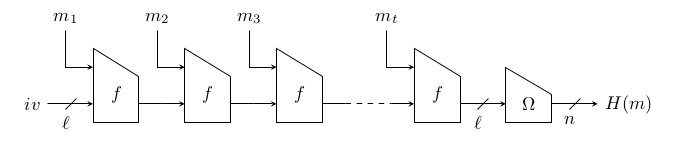
\includegraphics[width=5.5in]{groestlhashfunction.jpg}
    \end{center}
    \caption{Gr{\o}stl hash function \cite{00019}}
    \label{fig:lab}
  \end{figure}

  After the last message block is processed, the last chaining value output is sent through a $\Omega$ function, to get
  the hash output H(M).
  \begin{center}$H(M) = \Omega(h_{t}),$\end{center}
  The entire process is shown in the above figure 3.1.

  The f function shown above, is composed of two l-bit permutations called P and Q, which is defined as follows.
  \begin{center}$f(h, m) = P(h \oplus m) \oplus Q(m) \oplus h.$\end{center}
  
  \begin{figure}[h]
    \begin{center}
      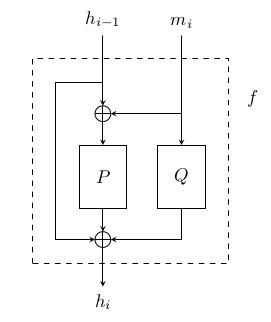
\includegraphics[width=2.5in]{groestlPQfunction.jpg}
    \end{center}
    \caption{Compression functions, where P and Q are $l-bit$ permutations \cite{00019}}
    \label{fig:lab}
  \end{figure}

  The $\Omega$ function consists of a $trunc_{n}(x)$ that outputs only the trailing n bits of input x. The $\Omega$ function
  can now be defined as 
  \begin{center}$\Omega(x) = trunc_{n}( P(x) \oplus x ).$\end{center}

  \begin{figure}[h]
    \begin{center}
      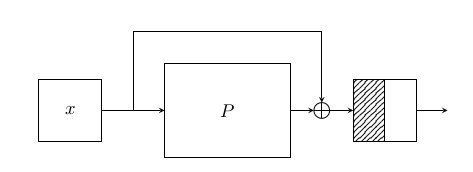
\includegraphics[width=4.5in]{groestlomegafunction.jpg}
    \end{center}
    \caption{Omega truncation function \cite{00019}}
    \label{fig:lab}
  \end{figure}

  In order to fit the varying input length message to the block sizes of $ l $ padding is defined. First bit '1' is
  appended, then $ w = -N - 65 \thickspace mod \thickspace l $ 0 bits are appended; where N is the length of the
  original message. Finally a 64 bit representation of $(N + w + 65) / l $. Given the need for message length, the
  maximum size of message digest in bits for Gr{\o}stl-512 version is $2^{73}-577$ bits, and that for 1024 version
  is $2^{74}-1089$bits.

  \subsection{Design of P and Q permutations}

  There are two variations for P and Q permutations, one each for the digest size lower and higher than 256 bits. There
  are four round transformations, that compose a round R. The permutation consists of a number of rounds R. R can be
  represented as 
  \begin{center}$ R = MixBytes \cdot ShiftBytes \cdot SubBytes \cdot AddRoundConstant $ \end{center}
  The transformations SubBytes and MixBytes are same for all transformation while, ShiftBytes and AddRoundConstant differ
  for each of the transformations. The transformations operate on matrix of bytes, with the permutation of lower size
  digest having matrix of 8 rows and 8 columns, while that for larger variant is of 16 columns and 8 rows. The mapping of
  the input to the state and the transformations are explained below. The number of rounds for each R is given as 
  recommendation in table 3.1 and the initial values are given in table 3.2
  
  \begin{table}
    \begin{center}
      \begin{tabular}{ *{3}{c} } \hline
        Permutations            & Digest size & Recommended value of r \\ \hline
        $P_{512}$ and $Q_{512}$   & 8 - 256     & 10 \\
        $P_{1024}$ and $Q_{1024}$ & 264 - 512   & 14 \\ \hline 
      \end{tabular}
      \caption{Recommended number of rounds\cite{00019}}
    \end{center}
  \end{table}

  \begin{table}
    \begin{center}
      \begin{tabular}{ *{2}{c} } \hline
        n   & $iv_{n}$         \\ \hline
        224 & 00 $\dots$ 00 00 e0 \\
        256 & 00 $\dots$ 00 01 00 \\
        384 & 00 $\dots$ 00 01 80 \\
        512 & 00 $\dots$ 00 02 00 \\ \hline
      \end{tabular}
    \caption{Initial values for Gr{\o}stl-n function. The numbers on left denote digest size in bits.\cite{00019}}
    \end{center}
  \end{table}


  \begin{itemize}
    \item {\bf Mapping:} of a 64-byte sequence of 00 01 02 $\ldots$ 3f to a 8 $\times$ 8 matrix is shown in the following matrix.
    For a 8 $\times$ 16 matrix, the mapping is extended the same way. Mapping the intermediate state values to byte sequence
    would be reverse of this.
      $ Input Mapping = \begin{bmatrix}
        00 & 08 & 10 & 18 & 20 & 28 & 30 & 38 \\
        01 & 09 & 11 & 19 & 21 & 29 & 31 & 39 \\
        02 & 0a & 12 & 1a & 22 & 2a & 32 & 3a \\
        03 & 0b & 13 & 1b & 23 & 2b & 33 & 3b \\
        04 & 0c & 14 & 1c & 24 & 2c & 34 & 3c \\
        05 & 0d & 15 & 1d & 25 & 2d & 35 & 3d \\
        06 & 0e & 16 & 1e & 26 & 2e & 36 & 3e \\
        07 & 0f & 17 & 1f & 27 & 2f & 37 & 3f
      \end{bmatrix}$
    \item {\bf AddRoundConstant:} transformation round XOR a round dependant constant to the state matrix say A. It is
    represented as $A \gets A \oplus C[i]$, where C[i] is the round constant in round i. The constants for both P and Q for both
    variations are given below.

    $ P_{512}: C[i] = \begin{bmatrix}
      00 \oplus i & 10 \oplus i & 20 \oplus i & 30 \oplus i & 40 \oplus i & 50 \oplus i & 60 \oplus i & 70 \oplus i \\
      00     & 00     & 00     & 00     & 00     & 00     & 00     & 00     \\
      00     & 00     & 00     & 00     & 00     & 00     & 00     & 00     \\
      00     & 00     & 00     & 00     & 00     & 00     & 00     & 00     \\
      00     & 00     & 00     & 00     & 00     & 00     & 00     & 00     \\
      00     & 00     & 00     & 00     & 00     & 00     & 00     & 00     \\
      00     & 00     & 00     & 00     & 00     & 00     & 00     & 00     \\
      00     & 00     & 00     & 00     & 00     & 00     & 00     & 00     \\
    \end{bmatrix}$

    and 

    $Q_{512}: C[i] = \begin{bmatrix}
      ff     & ff     & ff     & ff     & ff     & ff     & ff     & ff     \\
      ff     & ff     & ff     & ff     & ff     & ff     & ff     & ff     \\
      ff     & ff     & ff     & ff     & ff     & ff     & ff     & ff     \\
      ff     & ff     & ff     & ff     & ff     & ff     & ff     & ff     \\
      ff     & ff     & ff     & ff     & ff     & ff     & ff     & ff     \\
      ff     & ff     & ff     & ff     & ff     & ff     & ff     & ff     \\
      ff     & ff     & ff     & ff     & ff     & ff     & ff     & ff     \\
      ff \oplus i & ef \oplus i & df \oplus i & cf \oplus i & bf \oplus i & af \oplus i & 9f \oplus i & 8f \oplus i 
    \end{bmatrix}$

    Similarly, the P and Q for the wider variants are written.

    $ P_{1024}: C[i] = \begin{bmatrix}
      00 \oplus i & 10 \oplus i & 20 \oplus i & 30 \oplus i & 40 \oplus i & 50 \oplus i & 60 \oplus i & 70 \oplus i \ldots f0 \oplus i \\
      00     & 00     & 00     & 00     & 00     & 00     & 00     & 00     \dots 00 \\
      00     & 00     & 00     & 00     & 00     & 00     & 00     & 00     \dots 00 \\
      00     & 00     & 00     & 00     & 00     & 00     & 00     & 00     \dots 00 \\
      00     & 00     & 00     & 00     & 00     & 00     & 00     & 00     \dots 00 \\
      00     & 00     & 00     & 00     & 00     & 00     & 00     & 00     \dots 00 \\
      00     & 00     & 00     & 00     & 00     & 00     & 00     & 00     \dots 00 \\
      00     & 00     & 00     & 00     & 00     & 00     & 00     & 00     \dots 00 \\
    \end{bmatrix}$

    and 

    $Q_{1024}: C[i] = \begin{bmatrix}
      ff     & ff     & ff     & ff     & ff     & ff     & ff     & ff     \dots ff    \\
      ff     & ff     & ff     & ff     & ff     & ff     & ff     & ff     \dots ff    \\
      ff     & ff     & ff     & ff     & ff     & ff     & ff     & ff     \dots ff    \\
      ff     & ff     & ff     & ff     & ff     & ff     & ff     & ff     \dots ff    \\
      ff     & ff     & ff     & ff     & ff     & ff     & ff     & ff     \dots ff    \\
      ff     & ff     & ff     & ff     & ff     & ff     & ff     & ff     \dots ff    \\
      ff     & ff     & ff     & ff     & ff     & ff     & ff     & ff     \dots ff    \\
      ff \oplus i & ef \oplus i & df \oplus i & cf \oplus i & bf \oplus i & af \oplus i & 9f \oplus i & 8f \oplus i \dots 0f \oplus i
    \end{bmatrix}$

    where i is the round number represented as 8 bits value, and all other numbers are represented as
    hexadecimals.
    
\begin{table}
\begin{center}
  \begin{tabular}{ c | *{16}{c}}
     & 00 & 01 & 02 & 03 & 04 & 05 & 06 & 07 & 08 & 09 & 0a & 0b & 0c & 0d & 0e & 0f \\ \hline
  00 & 63 & 7c & 77 & 7b & f2 & 6b & 6f & c5 & 30 & 01 & 67 & 2b & fe & d7 & ab & 76 \\ 
  10 & ca & 82 & c9 & 7d & fa & 59 & 47 & f0 & ad & d4 & a2 & af & 9c & a4 & 72 & c0 \\
  20 & b7 & fd & 93 & 26 & 36 & 3f & f7 & cc & 34 & a5 & e5 & f1 & 71 & d8 & 31 & 15 \\
  30 & 04 & c7 & 23 & c3 & 18 & 96 & 05 & 9a & 07 & 12 & 80 & e2 & eb & 27 & b2 & 75 \\
  40 & 09 & 83 & 2c & 1a & 1b & 6e & 5a & a0 & 52 & 3b & d6 & b3 & 29 & e3 & 2f & 84 \\
  50 & 53 & d1 & 00 & ed & 20 & fc & b1 & 5b & 6a & cb & be & 39 & 4a & 4c & 58 & cf \\
  60 & d0 & ef & aa & fb & 43 & 4d & 33 & 85 & 45 & f9 & 02 & 7f & 50 & 3c & 9f & a8 \\
  70 & 51 & a3 & 40 & 8f & 92 & 9d & 38 & f5 & bc & b6 & da & 21 & 10 & ff & f3 & d2 \\
  80 & cd & 0c & 13 & ec & 5f & 97 & 44 & 17 & c4 & a7 & 7e & 3d & 64 & 5d & 19 & 73 \\
  90 & 60 & 81 & 4f & dc & 22 & 2a & 90 & 88 & 46 & ee & b8 & 14 & de & 5e & 0b & db \\
  a0 & e0 & 32 & 3a & 0a & 49 & 06 & 24 & 5c & c2 & d3 & ac & 62 & 91 & 95 & e4 & 79 \\
  b0 & e7 & c8 & 37 & 6d & 8d & d5 & 4e & a9 & 6c & 56 & f4 & ea & 65 & 7a & ae & 08 \\
  c0 & ba & 78 & 25 & 2e & 1c & a6 & b4 & c6 & e8 & dd & 74 & 1f & 4b & bd & 8b & 8a \\
  d0 & 70 & 3e & b5 & 66 & 48 & 03 & f6 & 0e & 61 & 35 & 57 & b9 & 86 & c1 & 1d & 9e \\
  e0 & e1 & f8 & 98 & 11 & 69 & d9 & 8e & 94 & 9b & 1e & 87 & e9 & ce & 55 & 28 & df \\
  f0 & 8c & a1 & 89 & 0d & bf & e6 & 42 & 68 & 41 & 99 & 2d & 0f & b0 & 54 & bb & 16 \\
  \end{tabular}
  \caption{Gr{\o}stl S-box. For an input x, you do a logical AND of x with f0 and with 0f.
  The first value obtained is used for column location and second for row location. The
  row and column location is used to identify the cell that will be used for substitution.
  \cite{00019}}
  \label{table:Groestlsbox}
\end{center}
\end{table}

  \item {\bf SubBytes:} substitutes each byte in state by value from S-box shown in table 3.3.
  Say $a_{i,j}$ a element in row i and column j of the state matrix, then the transformation done is 
  $a_{i,j} \gets S( a_{i,j}),  0 \leq i < 8, 0 \leq j < v.$ 
  
  \begin{figure}
    \begin{center}
      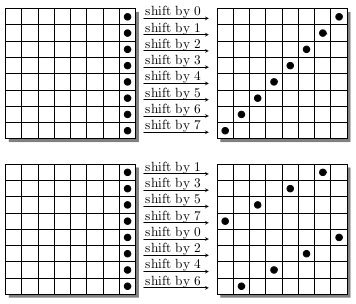
\includegraphics[width=3.6in]{groestl512shift.jpg}
    \end{center}
    \caption{ShiftBytes transformation of permutation $P_{512}$(top) and $Q_{512}$(bottom)\cite{00019}}
    \label{fig:lab}
  \end{figure}

  \item {\bf ShiftBytes:} transformation cyclically shifts the bytes in a row to left by that number. Let list 
  vector of a number denote the shift, with the index of the element indicating the row. The vector representation
  for $P_{512}$ = [0, 1, 2, 3, 4, 5, 6, 7] and $Q_{512}$ = [1, 3, 5, 7, 0, 2, 4, 6]. The shift is shown in figure
  3.4. Those for the larger permutation are $P_{1024}$ = [0, 1, 2, 3, 4, 5, 6, 11]and $Q_{1024}$ = 
  [1, 3, 5, 11, 0, 2, 4, 6]. This shifting is shown in figure 3.5.
    
  \begin{figure}
    \begin{center}
      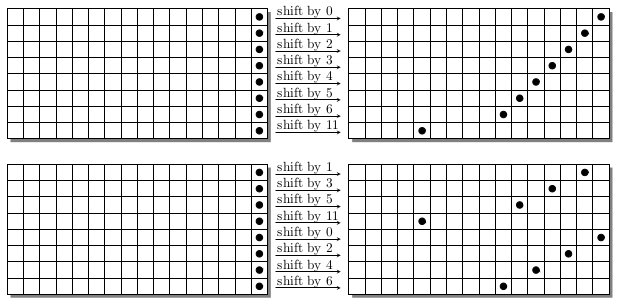
\includegraphics[width=6.4in]{groestl1024shift.jpg}
    \end{center}
    \caption{ShiftBytes transformation of permutation $P_{1024}$(top) and $Q_{1024}$(bottom)\cite{00019}}
    \label{fig:lab}
  \end{figure}

  $B = \begin{bmatrix}
  02 & 02 & 03 & 04 & 05 & 03 & 05 & 07 \\
  07 & 02 & 02 & 03 & 04 & 05 & 03 & 05 \\
  05 & 07 & 02 & 02 & 03 & 04 & 05 & 03 \\
  03 & 05 & 07 & 02 & 02 & 03 & 04 & 05 \\
  05 & 03 & 05 & 07 & 02 & 02 & 03 & 04 \\
  04 & 05 & 03 & 05 & 07 & 02 & 02 & 03 \\
  03 & 04 & 05 & 03 & 05 & 07 & 02 & 02 \\
  02 & 03 & 04 & 05 & 03 & 05 & 07 & 02 \\
  \end{bmatrix}$
  
  \item {\bf MixBytes:} transformation, multiplies each column of the state matrix A, by a constant 8 $\times$ 8 matrix B.
  The transformation, can be shown as $ A \gets B \times A$. The matrix B, can be seen as a finite field over $\mathbb{F}_{256}$.
  This finite field is defined over $\mathbb{F}_{2}$ by the irreducible polynomial $x^{8} \oplus x^{4} \oplus x^{3} \oplus x \oplus 1$.
  The mix bytes matrix B is shown above.
  % The composition of matrix B is shown, in appendix A, in item 2.
  %The bytes of the state matrix are in $\mathbb{F}_{256}$ in polynomials of degree at most 7, and coefficients in 0 and 1.
  %The matrix B, is circular shifting of the same row. Each row of the matrix below the current row, is rotated left by
  %a place.

  \end{itemize}

\section{BLAKE} 

BLAKE\cite{00002} hash function is built on HAIFA (HAsh Iterative FrAmework) structure \cite{00020} which is an improved
version of Merkle-Damg\.{a}rd function. And provides resistance to long-message second pre-image attack as well as
provides a salting option, that BLAKE uses\cite{00021}.
The design is local wide-pipe which avoids internal collisions. The compression function in BLAKE is tweaked version of 
ChaCha, a stream cipher. 

\begin{table}[h]
  \begin{center}
    \begin{tabular}{ *{6}{c} } \hline
      Algorithm & Word & Message    & Block & Digest & Salt \\ \hline
      BLAKE-224 & 32   & $< 2^{64}$  & 512   & 224    & 128  \\
      BLAKE-256 & 32   & $< 2^{64}$  & 512   & 256    & 128  \\
      BLAKE-384 & 64   & $< 2^{128}$ & 1024  & 384    & 256  \\
      BLAKE-512 & 64   & $< 2^{128}$ & 1024  & 512    & 256  \\ \hline
    \end{tabular}
    \caption{Specification of available input, output, block and salt sizes for various BLAKE hash functions.\cite{00002}}
  \end{center}
\end{table}

\begin{figure}[h]
  \begin{center}
    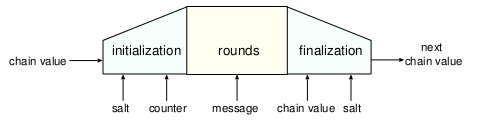
\includegraphics[width=4.75in]{blakelocalwidepipeconstruction.jpg}
  \end{center}
  \caption{Local wide construction of BLAKE's compression function\cite{00002}}
  \label{fig:lab}
\end{figure}

As seen from table 3.3, BLAKE has 4 variations of the algorithm that can give only 4 different digest lengths. The input
length is also smaller than Gr{\o}stl. Figure 3.6 shows how the individual message blocks are consumed. The construction
takes in 4 inputs, one message; two a salt, that makes function that parameter specific; and three a counter, which is 
count of all the bits hashed till then; and lastly a chaining value which is input of the previous operation or initial
value in case of hash initiation. The compression function is composed of a 4 $\times$ 4 matrix of words. Where one word is 
equal to 32 bits for BLAKE-256 variant, while 64 bit for variant BLAKE-512.

\begin{table}[h]
  \begin{center}
    \begin{tabular}{ c l } \hline
      Symbol                  & Meaning \\ \hline
      $\gets$                 & variable assignment \\
      $+$                     & addition modulo $2^{32}$ or (modulo $2^{64}$) \\
      $\ggg k$                & rotate k bits to least significant bits \\
      %$\ll k$                 & rotate k bits to most significant bits \\
      $\langle l \rangle_{k}$ & encoding of integer $l$ over $k$ bits \\ \hline
    \end{tabular}
    \caption{Convention of symbols used in BLAKE algorithm}
  \end{center}
\end{table}

\subsection{ BLAKE-256 }

The compression function takes following as input
\begin{itemize}
  \item a chaining value of $h = h_{0},\dots, h_{7}$
  \item a message block $m = m_{0},\dots, m_{15}$
  \item a salt $s = s_{0},\dots, s_{3}$
  \item a counter $t = t_{0}, t_{1}$
\end{itemize}
These four inputs of 30 words or 120 bytes, are processed as $h' = compress(h, m, s, t)$ to provide a new
chain value of 8 words.

  \subsubsection{Compression function}

  \begin{itemize}
    \item {\bf Constants}
      \begin{table}[h]
        \begin{center}
          \begin{tabular}{ *{4}{c}}
            $IV_{0}$ = 6A09E667 & $IV_{1}$ = BB67AE85 & $IV_{2}$ = 3C6EF372 & $IV_{3}$ = A54FF53A \\
            $IV_{4}$ = 510E527F & $IV_{5}$ = 9B05688C & $IV_{6}$ = 1F83D9AB & $IV_{7}$ = 5BE0CD19 \\
          \end{tabular}
          \caption{Initial values which become the chaining value for the first message block\cite{00002}}
        \end{center}
      \end{table}
      
      \begin{table}[h]
        \begin{align*}
             {\tt c_{0}}  &= {\tt 243F6A88} & {\tt c_{1}}  &= {\tt 85A308D3} & {\tt c_{2}}  &= {\tt 13198A2E} & {\tt c_{3}}  &= {\tt 03707344}
          \\ {\tt c_{4}}  &= {\tt A4093822} & {\tt c_{5}}  &= {\tt 299F31D0} & {\tt c_{6}}  &= {\tt 082EFA98} & {\tt c_{7}}  &= {\tt EC4E6C89} 
          \\ {\tt c_{8}}  &= {\tt 452821E6} & {\tt c_{9}}  &= {\tt 38D01377} & {\tt c_{10}} &= {\tt BE5466CF} & {\tt c_{11}} &= {\tt 34E90C6C} 
          \\ {\tt c_{12}} &= {\tt C0AC29B7} & {\tt c_{13}} &= {\tt C97C50DD} & {\tt c_{14}} &= {\tt B5470917} & {\tt c_{15}} &= {\tt 3F84D5B5} 
        \end{align*}
        \caption{16 constants used for BLAKE-256\cite{00002}}
      \end{table}

      \begin{table}
        \begin{center}
          \begin{tabular}{ c| *{16}{c}} \hline
            $\sigma_{0}$ & 0  & 1  & 2  & 3  & 4  & 5  & 6  & 7  & 8  & 9  & 10 & 11 & 12 & 13 & 14 & 15 \\
            $\sigma_{1}$ & 14 & 10 & 4  & 8  & 9  & 15 & 13 & 6  & 1  & 12 & 0  & 2  & 11 & 7  & 5  & 3  \\
            $\sigma_{2}$ & 11 & 8  & 12 & 0  & 5  & 2  & 15 & 13 & 10 & 14 & 3  & 6  & 7  & 1  & 9  & 4  \\
            $\sigma_{3}$ & 7  & 9  & 3  & 1  & 13 & 12 & 11 & 14 & 2  & 6  & 5  & 10 & 4  & 0  & 15 & 8  \\
            $\sigma_{4}$ & 9  & 0  & 5  & 7  & 2  & 4  & 10 & 15 & 14 & 1  & 11 & 12 & 6  & 8  & 3  & 13 \\
            $\sigma_{5}$ & 2  & 12 & 6  & 10 & 0  & 11 & 8  & 3  & 4  & 13 & 7  & 5  & 15 & 14 & 1  & 9  \\
            $\sigma_{6}$ & 12 & 5  & 1  & 15 & 14 & 13 & 4  & 10 & 0  & 7  & 6  & 3  & 9  & 2  & 8  & 11 \\
            $\sigma_{7}$ & 13 & 11 & 7  & 14 & 12 & 1  & 3  & 9  & 5  & 0  & 15 & 4  & 8  & 6  & 2  & 10 \\
            $\sigma_{8}$ & 6  & 15 & 14 & 9  & 11 & 3  & 0  & 8  & 12 & 2  & 13 & 7  & 1  & 4  & 10 & 5  \\
            $\sigma_{9}$ & 10 & 2  & 8  & 4  & 7  & 6  & 1  & 5  & 15 & 11 & 9  & 14 & 3  & 12 & 13 & 0  \\ \hline
          \end{tabular}
          \caption{Round permutations to be used\cite{00002}}
        \end{center}
      \end{table}
    
    \item {\bf Initialization: } The constants mentioned are used with the salts, and counter along with initial
    value used as chaining input, to create a initial matrix of 4 $\times$ 4, 16 word state.

    \begin{center}
    $\begin{pmatrix} v_{0} & v_{1} & v_{2} & v_{3} \\ v_{4} & v_{5} & v_{6} & v_{7} \\
                     v_{8} & v_{9} & v_{10} & v_{11} \\ v_{12} & v_{13} & v_{14} & v_{15}\end{pmatrix} 
    \gets
    \begin{pmatrix} h_{0} & h_{1} & h_{2} & h_{3} \\ h_{4} & h_{5} & h_{6} & h_{7} \\
       s_{0} \oplus c_{0} & s_{1} \oplus c_{1} & s_{2} \oplus c_{2} & s_{3} \oplus c_{3} \\ 
       t_{0} \oplus c_{4} & t_{0} \oplus c_{5} & t_{1} \oplus c_{6} & t_{1} \oplus c_{7} \end{pmatrix}$
    \end{center}

    \item {\bf Round function:} After initialisation, the state is subjected to column and diagonal operations, 14
    times. A round operation G acts as per following

    \begin{table}
      \begin{center}
        \begin{tabular}{ *{4}{c}}
        $ G_{0}(v_{0}, v_{8}, v_{12})$ & $G_{1}(v_{1}, v_{5}, v_{9}, v_{13})$ & $G_{2}(v_{2}, v_{6}, v_{10}, v_{14})$ & $G_{3}(v_{3}, v_{7}, v_{11}, v_{15}) $\\
 $G_{4}(v_{0}, v_{5}, v_{10}, v_{15})$ & $G_{5}(v_{1}, v_{6}, v_{11}, v_{12})$ & $G_{6}(v_{2}, v_{7}, v_{8}, v_{13})$ & $G_{7}(v_{3}, v_{4}, v_{9}, v_{14})$
        \end{tabular}
      \end{center}
    \end{table}

    %$ G_{0}(v_{0}, v_{8}, v_{12}) \; G_{1}(v_{1}, v_{5}, v_{9}, v_{13}) \; G_{2}(v_{2}, v_{6}, v_{10}, v_{14}) \; G_{3}(v_{3}, v_{7}, v_{11}, v_{15}) \\
    %G_{4}(v_{0}, v_{5}, v_{10}, v_{15}) \; G_{5}(v_{1}, v_{6}, v_{11}, v_{12}) \; G_{6}(v_{2}, v_{7}, v_{8}, v_{13}) \; G_{7}(v_{3}, v_{4}, v_{9}, v_{14})$

    where the round function $G_{i}(a, b, c, d)$ sets

    \newpage
    
    $
    a \gets a + b + (m_{\sigma_{r}(2i)} \oplus c_{\sigma_{r}(2i + 1)}) \\
    d \gets (d \oplus a) \ggg 16 \\
    c \gets c + d \\
    b \gets (b \oplus c) \ggg 12 \\
    a \gets a + b + (m_{\sigma_{r}(2i + 1)} \oplus c_{\sigma_{r}(2i)}) \\
    d \gets (d \oplus a) \ggg 8 \\
    c \gets c + d \\
    b \gets (b \oplus c) \ggg 7
    $

    The implementation of the G function is shown below.
    \begin{figure}[h]
      \begin{center}
        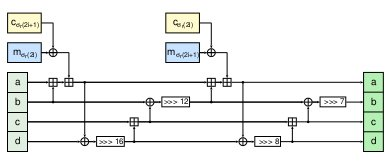
\includegraphics[width=4in]{blakeGfunction.jpg}
      \end{center}
      \caption{The $G_{i}$ function in BLAKE\cite{00002}}
      \label{fig:lab}
    \end{figure}

    \item {\bf Finalization:} The chaining values for the next stage are obtained by XOR of the words from the state 
    matrix, the salt and the initial value.

    $
    h'_{0} \gets h_{0} \oplus s_{0} \oplus v_{0} \oplus v_{8} \\
    h'_{1} \gets h_{1} \oplus s_{1} \oplus v_{1} \oplus v_{9} \\
    h'_{2} \gets h_{2} \oplus s_{2} \oplus v_{2} \oplus v_{10} \\
    h'_{3} \gets h_{3} \oplus s_{3} \oplus v_{3} \oplus v_{11} \\
    h'_{4} \gets h_{4} \oplus s_{0} \oplus v_{4} \oplus v_{12} \\
    h'_{5} \gets h_{5} \oplus s_{1} \oplus v_{5} \oplus v_{13} \\
    h'_{6} \gets h_{6} \oplus s_{2} \oplus v_{6} \oplus v_{14} \\
    h'_{7} \gets h_{7} \oplus s_{3} \oplus v_{7} \oplus v_{15} \\
    $
  \end{itemize}

  \subsubsection{Hashing the message}

  A given input message is padded with a bit '1' followed followed by at most 511 bits of zeros, so that the message 
  size is equal to 447 modulo 512. This padding is followed by a bit '1' and a 64-bit unsigned big-endian representation
  of block length $l$. The padding to a message, can be represented as $m \gets m \parallel 1000 \dots 0001\langle l \rangle_{64}$

  \begin{algorithm}
  \caption{BLAKE Compression procedure\cite{00002}}
  \begin{algorithmic}[1]
    \State $ h^{0} \gets IV $
    \For {$i = 0,\dots, N - 1$}
      \State $h^{i+1} \gets compress(h^{i}, m^{i}, s, l^{i})$
    \EndFor
    \State\Return{$h^{N}$}
  \end{algorithmic}
  \end{algorithm}

  As shown in algorithm 3.1, the BLAKE compression function ingests the padded message block by block, in a loop 
  starting from the initial value, and then sends the last chained value obtained from the finalization to the 
  $\Omega$ truncation function, to obtain the hash value.

\subsection{BLAKE-512}

operates on 64-bit words and returns a 64-byte hash value. The chaining value is 512 bit long, message blocks are
1024 bits, salt is 256 bits, and counter size is 128 bits. The difference from BLAKE-256 are in constants(tables 3.8 
and 3.9), compression function and the way message is padded.

  \begin{table}
    \begin{align*}
      {\tt IV_{0}} &= {\tt 6A09E667F3BCC908} & {\tt IV_{1}} &= {\tt BB67AE8584CAA73B} & {\tt IV_{2}} &= {\tt 3C6EF372FE94F82B} \\
      {\tt IV_{3}} &= {\tt A54FF53A5F1D36F1} & {\tt IV_{4}} &= {\tt 510E527FADE682D1} & {\tt IV_{5}} &= {\tt 9B05688C2B3E6C1F} \\
      {\tt IV_{6}} &= {\tt 1F83D9ABFB41BD6B} & {\tt IV_{7}} &= {\tt 5BE0CD19137E2179} &                                        \\      
    \end{align*}
    \caption{Initial values used for BLAKE-512\cite{00002}}
  \end{table}
  
  \begin{table}
    \begin{align*}
         {\tt c_{0}}  &= {\tt 243F6A8885A308D3} & {\tt c_{1}}  &= {\tt 13198A2E03707344} & {\tt c_{2}}  &= {\tt A4093822299F31D0} 
      \\ {\tt c_{3}}  &= {\tt 082EFA98EC4E6C89} & {\tt c_{4}}  &= {\tt 452821E638D01377} & {\tt c_{5}}  &= {\tt BE5466CF34E90C6C} 
      \\ {\tt c_{6}}  &= {\tt C0AC29B7C97C50DD} & {\tt c_{7}}  &= {\tt 3F84D5B5B5470917} & {\tt c_{8}}  &= {\tt 9216D5D98979FB1B} 
      \\ {\tt c_{9}}  &= {\tt D1310BA698DFB5AC} & {\tt c_{10}} &= {\tt 2FFD72DBD01ADFB7} & {\tt c_{11}} &= {\tt B8E1AFED6A267E96} 
      \\ {\tt c_{12}} &= {\tt BA7C9045F12C7F99} & {\tt c_{13}} &= {\tt 24A19947B3916CF7} & {\tt c_{14}} &= {\tt 0801F2E2858EFC16} 
      \\ {\tt c_{15}} &= {\tt 636920D871574E69} &                                        &      
    \end{align*}
    \caption{16 constants used for BLAKE-512\cite{00002}}
  \end{table}
  
  Compression function in BLAKE-512 gets 16 iterations instead of 14 as in BLAKE-256, as well the rotations
  are updated and word size increased from 32 bits to 64 bits. The $G_{i}(a, b, c, d)$ 
  is given as 

  $
  a \gets a + b + (m_{\sigma_{r}(2i)} \oplus c_{\sigma_{r}(2i + 1)}) \\
  d \gets (d \oplus a) \ggg 32 \\
  c \gets c + d \\
  b \gets (b \oplus c) \ggg 25 \\
  a \gets a + b + (m_{\sigma_{r}(2i + 1)} \oplus c_{\sigma_{r}(2i)}) \\
  d \gets (d \oplus a) \ggg 16 \\
  c \gets c + d \\
  b \gets (b \oplus c) \ggg 11
  $
  
  Once more than 9 rounds are done, the permutation table rules kick in, for example if round r \textgreater 9 then
  permutation used is $\sigma_{r \thickspace mod \thickspace 10}$, say r = 15 then permutation would be 
  $\sigma_{15 \thickspace mod \thickspace 10} = \sigma_{5}$.

  For the padding, the message is first padded with bit 1 and then as many zeros required to make the bit length
  equivalent to 895 modulo 1024. After that another bit of value 1 is appended followed by 128-bits unsigned big-endian
  representation of of message length as $m \gets m \parallel 100 \dots 001 \langle l \rangle_{128}$.

\subsection{BLAKE-224 and BLAKE-384}

  \subsubsection{BLAKE-224}
  BLAKE-224 is similar to BLAKE-256, but differs slightly. It has different initial values, different padding and the
  output bits are truncated to first 224 bits.
  \begin{table}[h]
    \begin{center}
      \begin{tabular}{ *{4}{c}}
        $IV_{0}$ = C1059ED8 & $IV_{1}$ = 367CD507 & $IV_{2}$ = 3070DD17 & $IV_{3}$ = F70E5939 \\
        $IV_{4}$ = FFC00B31 & $IV_{5}$ = 68581511 & $IV_{6}$ = 64F98FA7 & $IV_{7}$ = BEFA4FA4 \\
      \end{tabular}
      \caption{Initial values for BLAKE-224 which are taken from SHA-224\cite{00002}}
    \end{center}
  \end{table}
  The padding differs from BLAKE-256 in way that the bit preceding the message length is replaced by a 0 bit. Which
  is represented as $m \gets m \parallel 100 \dots 000 \langle l \rangle_{64}$.

  \subsubsection{BLAKE-384}
  In BLAKE-384 the output of BLAKE-512 is truncated to 384 bits. The padding differs from BLAKE-512, in way that bit
  preceding the length encoding is 0 and not 1. It can be shown as $m \gets m \parallel 100 \dots 000 \langle l \rangle_{128}$. The
  initial chaining values are given in table 3.11.
  \begin{table}[h]
    \begin{align*}
      {\tt IV_{0}} &= {\tt CBBB9D5DC1059ED8} & {\tt IV_{1}} &= {\tt 629A292A367CD507} & {\tt IV_{2}} &= {\tt 9159015A3070DD17} \\
      {\tt IV_{3}} &= {\tt 152FECD8F70E5939} & {\tt IV_{4}} &= {\tt 67332667FFC00B31} & {\tt IV_{5}} &= {\tt 8EB44A8768581511} \\
      {\tt IV_{6}} &= {\tt DB0C2E0D64F98FA7} & {\tt IV_{7}} &= {\tt 47B5481DBEFA4FA4} &                                        \\      
    \end{align*}
    \caption{Initial values for BLAKE-384\cite{00002}}
  \end{table}

\newpage

\section{Keccak}
Keccak hash function, is built on sponge construction, which can input and output arbitrary length strings. The sponge
construction has two phases. First is absorb, where the input message is ingested in blocks of defined bit rate interleaved
with the permutations. And the second phase is squeeze phase, where the blocks of output are squeezed out as per the 
bit rate blocks. The Keccak, state is different in the sense that, the permutations work on a 3 dimensional block, cube
structure rather than linear strings, or 2 dimensional arrays.

  \subsection{Keccak state, sponge functions and padding} 
  \begin{figure}[h]
    \begin{center}
      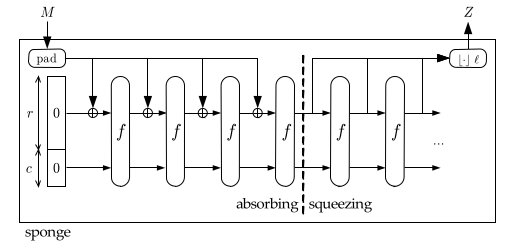
\includegraphics[width=5.5in]{keccakspongeconstruction.jpg}
    \end{center}
    \caption{Sponge construction $Z = Sponge[f, pad, r](M, l)$\cite{00016}}
    \label{fig:lab}
  \end{figure}

  The sponge construction is used to build function $SPONGE[f, pad, r]$ which inputs and outputs variable length strings 
  \cite{00016}. It uses fixed length permutation $f$, a padding "pad", and parameter bit rate 'r'. The permutations are 
  operated on fixed number of bits, width $b$. The value $c = b - r$ is the capacity of the sponge function. The width 
  $b$ in Keccak defines the state size which can be any of the following \{25, 50, 100, 200, 400, 800, 1600\} number of 
  bits. 
  
  \begin{figure}
    \begin{center}
      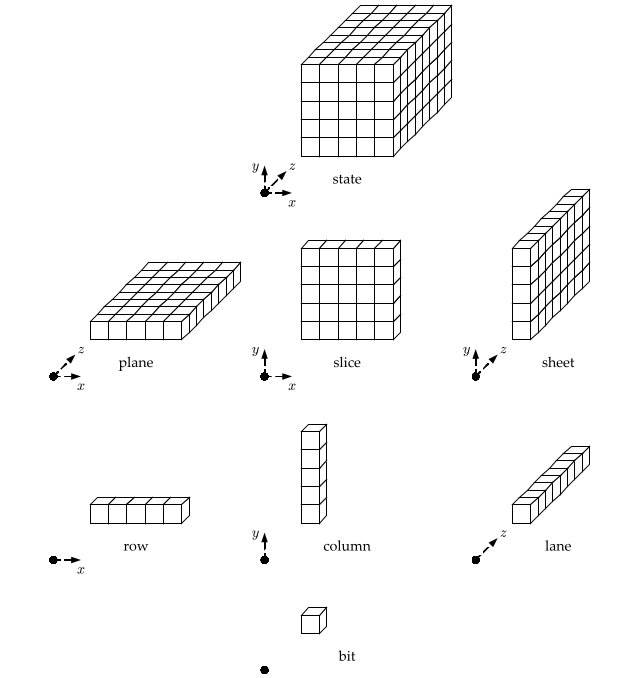
\includegraphics[width=6.5in]{keccakstateterminology.jpg}
    \end{center}
    \caption{Sponge construction $Z = Sponge[f, pad, r](M, l)$\cite{00015}}
    \label{fig:lab}
  \end{figure}

  The state in Keccak can be represented as a cube having bits, as shown in figure 3.9. The initial state to the sponge
  construction has value 'b' number of 0 bits(represented as $0^{b}$), and called the root state. The root state has fixed
  value and should not be considered as initial value to sponge construction. The different number of state produces
  the Keccak family of hash function variations denoted by $KECCAK-f[b]$.
  
  The varying number of states can be visualized as state having varying number or $l$ number of slices. The width $b$ is
  defined as $b = 25 \times 2^{l}$, where $l$ takes values from 0 to 6.
  
  \begin{algorithm}
    \caption{The sponge construction $SPONGE[f, pad, r]$\cite{00016}}
    \begin{algorithmic}[1]
      \Require $r < b$
      \State {\bf Interface:} Z = sponge($M, l$) with $M \in \mathbb{Z}^{*}_{2}$, integer $ l > 0$ and $Z \in \mathbb{Z}^{l}_{2}$
      \State $P = M \parallel pad[r](\mid M \mid)$
      \State $s = 0^{b}$
      \State \For {$i = 0 \thickspace to \mid P \mid_{r} - 1$}
        \State $s = s \oplus ( P_{i} \parallel 0^{b - r})$
        \State $s = f(s)$
      \State \EndFor
      \State $ Z = \lfloor s \rfloor_{r}$
      \State \While $\mid Z \mid_{r} r < l $
        \State $s = f(s)$
        \State $Z = Z \parallel \lfloor s \rfloor_{r}$
      \State \EndWhile
      \State \Return $\lfloor Z \rfloor_{l}$ 
    \end{algorithmic}
  \end{algorithm}

  Algorithm 3.2 shows how the sponge construction applied to $KECCAK-f[r + c]$, with multi-rate padding. In algorithm 3.2
  length of a string $M$ is denoted by $\mid M \mid $. The string $M$ can also be considered as having blocks of size say x,
  and those number of blocks are shown as $\mid M \mid_{x}$. The $\lfloor M \rfloor_{l}$ denotes the string $M$ truncated to its first $l$ bits.
  
  The multi-rate padding in Keccak is denoted as $pad \thickspace 1 0^{*}1$ , where a bit '1' is appended to message, followed 
  by minimum number of zeros. And lastly a single bit 1, so that resultant block is multiple of block length $b$. Thus 
  Keccak in terms of sponge function can be defined as 
  \begin{center}$KECCAK[r, c] \doteq SPONGE[KECCAK-f[r + c], pad1 0^{*}1, r]$ \end{center}
  Where $ r > 0$ and $r + c$ is the width. The default value of $r$ is $1600 - c$, and the default value of $c$ is 576.
  \begin{center}$KECCAK[c] \doteq KECCAK[r = 1600 - c, c],$\end{center}
  \begin{center}$KECCAK[] \doteq KECCAK[c = 576]$\end{center}
    
  \subsection{Permutations}

  The $KECCAK-f[b]$ permutations are operated on state represented as a[5][5][w], with w = $2^{l}$, where l can be any value
  from 0 to 6. The position in this 3 dimensional state is given by $a[x][y][z]$ where $x, y \in \mathbb{Z}_{5}$ and $z \in 
  \mathbb{Z}_{w}$. The mapping of the bits from the input message 's' to state 'a' is like this $s[w (5y + x) + z] = a[x][y][z]$.
  The $x, y$ coordinates are taken modulo 5, while the $z$ coordinate is taken as modulo $w$.  \cite{00015}

  There are five steps, for a permutation round R. 
  \begin{center}$R = \zeta \circ \chi \circ \pi \circ \rho \circ \theta$\end{center}
  The permutations are repeated for $12 + 2l$ times, with $l$ dependent on the variant chosen. \\
  \begin{align*}
    \theta &: a[x][y][z] & \gets & \thickspace a[x][y][z] + \displaystyle\sum\limits_{y' = 0}^{4} a[x - 1][y'][z] + \displaystyle\sum\limits_{y' = 0}^{4} a[x + 1][y'][z - 1], \\
    \rho &: a[x][y][z] & \gets & \thickspace a[x][y][z - (t + 1)(t + 2) / 2], \\
    & & & \thickspace t \thickspace satisfying \thickspace 0 \leq t < 24 \thickspace and \thickspace
    \begin{pmatrix} 0 & 1 \\ 2 & 3 \end{pmatrix}^{t} \begin{pmatrix} 1 \\ 0 \end{pmatrix} = \begin{pmatrix} x \\ y \end{pmatrix}
    in \thickspace GF(5)^{2 \times 2}, \\
    & & & \thickspace or \thickspace t = -1 \thickspace if \thickspace x = y = 0, \\
    \pi &: a[x][y] & \gets & \thickspace a[x'][y'], \thickspace with \thickspace
    \begin{pmatrix} x \\ y \end{pmatrix} = \begin{pmatrix} 0 & 1 \\ 2 & 3 \end{pmatrix} \begin{pmatrix} x' \\ y'\end{pmatrix}, \\
    \chi &: a[x] & \gets & \thickspace a[x] + (a[x + 1] + 1) \thickspace a[x + 2], \\
    \zeta &: a & \gets & \thickspace a + RC[i_{r}].
  \end{align*}

  The addition and the multiplications are in Galois field GF(2), except for the round constants $RC[i_{r}]$. The round constants 
  are given by
  \begin{center}$RC[i_{r}][0][0][2^{j} - 1] = rc[j + 7i_{r}]$ for all $ 0 \leq j \leq l$,\end{center}
  and the rest are zeros. The value of $rc[t] \in GF(2)$ is output of linear feedback shift register given as
  \begin{center}$rc[t] = (x^{t} \thickspace mod \thickspace x^{8} + x^{6} + x^{5} + x^{4} + 1)$ mod x in GF(2)[$x$].\end{center}

  \begin{figure}
    \begin{center}
      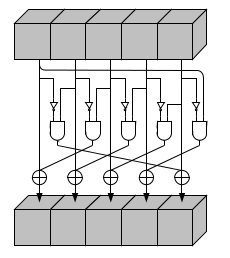
\includegraphics[width=2.3in]{keccakchi.jpg}
    \end{center}
    \caption{$\chi$ applied to a single row.\cite{00015}}
    \label{fig:lab}
  \end{figure}

  \begin{algorithm}
    \caption{ $\chi$ transformation KECCAK\cite{00015}}
    \begin{algorithmic}[1]
      \State \For {$y = 0 \thickspace to \thickspace 4$}
      \State \For {$x = 0 \thickspace to \thickspace 4$}
      $A[x, y] = a[x, y] \oplus ((NOT \thickspace a[x + 1, y]) \thickspace AND \thickspace a[x + 2, y])$
      \State \EndFor
      \State \EndFor
    \end{algorithmic}
  \end{algorithm}
  
  \begin{figure}
    \begin{center}
      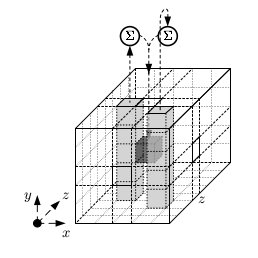
\includegraphics[width=2.7in]{keccaktheta.jpg}
    \end{center}
    \caption{$\theta$ applied to a single bit\cite{00015}}
    \label{fig:lab}
  \end{figure}

  \begin{algorithm}
    \caption{ $\theta$ transformation KECCAK\cite{00015}}
    \begin{algorithmic}[1]
      \State \For {$x = 0 \thickspace to \thickspace 4$}
      \State $C[x] = a[x, 0]$
      \State \For {$y = 1 \thickspace to \thickspace 4$}
      $C[x] = C[x] \oplus a[x, y]$
      \State \EndFor
      \State \EndFor
      \State \For {$x = 0 \thickspace to \thickspace 4$}
      \State $D[x] = C[x - 1] \oplus ROT(C[x + 1], 1)$
      \State \For {$y = 0 \thickspace to \thickspace 4$}
      \State $A[x, y] = a[x, y] \oplus D[x]$
      \State \EndFor
      \State \EndFor
    \end{algorithmic}
  \end{algorithm}

  \begin{algorithm}
    \caption{ $\pi$ transformation KECCAK\cite{00015}}
    \begin{algorithmic}[1]
      \State \For {$x = 0 \thickspace to \thickspace 4$}
      \State \For {$y = 1 \thickspace to \thickspace 4$}
      \State $\begin{pmatrix} X \\ Y \end{pmatrix} = \begin{pmatrix} 0 & 1 \\ 2 & 3 \end{pmatrix} \begin{pmatrix}x \\ y \end{pmatrix}$
      \State $A[X, Y] = a[x, y]$
      \State \EndFor
      \State \EndFor
    \end{algorithmic}
  \end{algorithm}

  \begin{figure}
    \begin{center}
      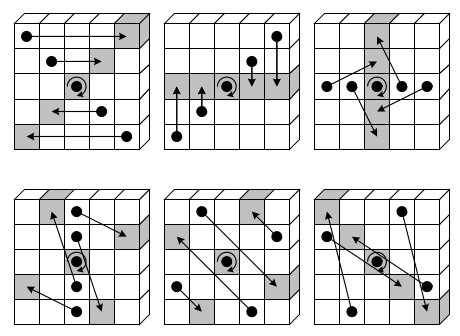
\includegraphics[width=4.75in]{keccakpi.jpg}
    \end{center}
    \caption{$\pi$ applied to a single slice\cite{00015}}
    \label{fig:lab}
  \end{figure}

  \begin{algorithm}
    \caption{ $\rho$ transformation KECCAK\cite{00015}}
    \begin{algorithmic}[1]
      \State $A[0, 0] = a[0, 0]$
      \State $\begin{pmatrix} x \\ y \end{pmatrix} = \begin{pmatrix} 1 \\ 0 \end{pmatrix}$
      \State \For{$t = 0 \thickspace to \thickspace 23$}
      \State $A[x, y] = ROT(a[x, y], (t + 1)(t + 2) / 2)$
      \State $\begin{pmatrix} x \\ y \end{pmatrix} = \begin{pmatrix} 0 & 1 \\ 2 & 3 \end{pmatrix} \begin{pmatrix}x \\ y \end{pmatrix}$
      \State \EndFor
    \end{algorithmic}
  \end{algorithm}

  \begin{figure}
    \begin{center}
      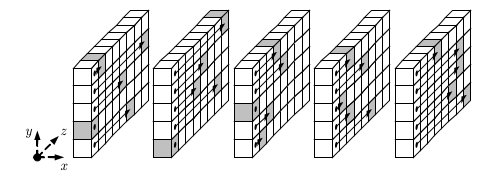
\includegraphics[width=5.1in]{keccakrho.jpg}
    \end{center}
    \caption{$\rho$ transformation applied to lanes\cite{00015}}
    \label{fig:lab}
  \end{figure}

  \begin{table}
    \begin{center}
      \begin{tabular}{ c | *{5}{c}}
                & $x = 2$ & $x = 4$ & $x = 0$ & $x = 1$ & $x = 2$ \\ \hline
        $y = 2$ & 153     & 231     & 3       & 10      & 171     \\
        $y = 1$ & 55      & 276     & 36      & 300     & 6       \\
        $y = 0$ & 28      & 91      & 0       & 1       & 190     \\
        $y = 4$ & 120     & 78      & 210     & 66      & 253     \\
        $y = 3$ & 21      & 136     & 105     & 45      & 15      \\
      \end{tabular}
      \caption{Offsets for $\rho$ transformation\cite{00015}}
    \end{center}
  \end{table}


%\chapter{Related work}

%From the wolfram alpha pages what is a field. A field is one that have field axioms of associativity, distributivity,
%commutativity, inverse, identity(else you cannot have the inverse). A field with finite elements or field order is finite
%or Galois field. GF(p) where the Galois field of order p. The order of the field is a power of a prime number. A GF 
%consists of residue classes of modulo p. Now a residue can be a congruence b mod n, then b is the residue. A finite
%field will have limited number of residues, which will form a residue class. The residue classes of a function x is
%all possible values of residue of f(x)(mod n). Galois fields are made of residues of the modulus function, so the 
%equivalence is based on the modulus function.

%OK, another thing, that I learned about in past few days was about Galois field. Why Galois field? Well, the thing
%is they are the building blocks to what is there in the cryptographic function. What did I learn about field, that
%number of elements in field are limited for the modulo of the prime that is the order of the field. Since it is
%modulo, so all the elements repeat with the numbers. The elements in a field obey the axioms of field that include
%associativity, distributive, commutative, inverse and identity. The modulo prime can be represented as a polynomial
%of odd powers summing to the power of the prime power of the field. The polynomial has to be irreducible, since if
%you allow reducible polynomial there is a possibility, that the polynomials would sum to the modulo and become a zero
%element that cannot be allowed to happen. Since multiplication with zero will be zero. Other than that, figuring
%out a inverse in field is hard but if you have the look up tables of logarithms with the generator numbers whose 
%successive powers modulo the prime generates all the numbers in the field. This table is then made as a look up,
%when you multiply the polynomials. There is a already algorithm and code written up for that thing. Which can be used.

%Well in this case in the first part the rant is about how not to get the security of the hash function not to be 
%based on the length of the message digest. Why so? Well then you cannot say anything about the security of the 
%function if the output of it changes from time to time. So you use the sponge function to make claims about the security.
%Please note in mind that they are saying that sponge is close to random oracle and only exception of internal
%collisions.

%\section{Zero Sum Distinguishers}
%Zero sum distinguishers were first presented in CHES 2009 rump session \cite{00014}. A zero sum distinguisher, for any
%function is a way to find a set of values, that sum to zero, such that their respective images also sum to zero.

\section{Cryptanalysis done on Keccak}

\subsection{Rotational cryptanalysis of round-reduced KECCAK} \cite{00022}
In this paper, Paweł Morawiecki, Josef Pierpzyk and Marian Srebrny apply rotational cryptanalysis to Keccak. 
They use it to construct a 5-round distinguisher for Keccak-f[1600] and to do preimage generation for 4 rounds of 
Keccak[r=1024,c=576] truncated to 512 bits with complexity 2506 calls to Keccak-f[1600].

\subsection{New Attacks on Keccak 224 and Keccak 256} \cite{00023}
The authors of this paper present practical-time collisions on Keccak[r=1088,c=512] (and lower capacity) with 4 rounds. 
They combine a low-weight trail over 3 rounds with algebraic techniques.

\subsection{Practical Analysis of Reduced Round Keccak} \cite{00024}
In this paper, the authors propose several practical-time attacks on the Keccak hash function with 2 to 4 rounds. 
First, they give a differential distinguisher exploiting a low-weight differential trail. Its complexity is 225 for 4 
rounds. Then, they show how to produce a collision (resp. near-collision) on 2 (resp. 3) rounds of Keccak[r=1088,c=512] 
(and lower capacity) with complexity 233 (resp. 225). Finally, they present an algorithm to find (second) preimages in 
time 231 and memory 229.

\subsection{Unaligned Rebound Attack: Application to Keccak} \cite{00025}
This paper analyzes two aspects of differential cryptanalysis on Keccak: efficient trails and rebound attacks. In the 
former, the authors propose a heuristic to build differential trails with a low restriction weight. For Keccak-f[1600], 
they obtained trails of weight 32, 142 and 709 for 3, 4 and 5 rounds, respectively. In the latter, the paper presents 
distinguishers making use of the rebound attack for up to 8 rounds of Keccak-f[1600] with a complexity of 2491.

\subsection{Improved zero-sum distinguisher for full round Keccak-f permutation} \cite{00026}
The authors of this paper noted a property of the inverse of the non-linear function χ: while χ-1 has algebraic degree 3,
the product of any two output bits also has degree 3. This allows to estimate the degree of the Keccak-f rounds more tightly 
and to extend the zero-sum distinguisher on Keccak-f[1600] to size 21575 for 24 rounds.

\subsection{A SAT-based preimage analysis of reduced Keccak hash functions} \cite{00027}
In this paper, Paweł Morawiecki and Marian Srebrny report on experiments for generating preimages using SAT solvers. 
They attack Keccak versions calling Keccak-f with width 50, 200 and 1600 and with a reduced number of rounds. 
They compare the SAT solver approach with plain exhaustive search and it turns out to be faster for up to 3 rounds.

\subsection{Zero-sum Distinguishers for Iterated Permutations and Application to Keccak-f and Hamsi-256} \cite{00028}
In this paper, Christina Boura and Anne Canteaut extend their zero-sum distinguishers to 20 rounds.

\section{Cryptanalysis done on BLAKE}
\section{Cryptanalysis done on Gr$\o$stl}

\chapter{Hypothesis based on Hill Climbing to find near collisions}

%% Obviously you need to delete these lines when you have written up your text
%\begin{itemize}
%\item{} How you designed your solution
%\item{} Rationale for decisions
%\item{} Compare and contrast design with other approaches (related work) 
%\end{itemize}

\section{Finding near collisions with Hill Climbing}

A generic algorithm applied to find collisions, in reduced rounds of some SHA-3 competitors was Hill Climbing
\cite{00029}. Near collisions in which more than 75\% of the bits were same for two different messages, were found 
for reduced rounds of BLAKE-32, Hamsi-256 and JH. Near collision results are important for knowing the security
margins. In some cases, output of hash functions may be truncated for compatibility or efficiency purposes. In 
such cases near collisions could be improved to obtain collisions.

A $\epsilon / n $ bit near collision for hash function h and two messages $M_{1}$ and $M_{2}$, where $M_{1} \neq M_{2}$ can be 
defined as
\begin{center}$HW( h( M_{1}, CV ) \oplus h( M_{2}, CV ) ) = n - \epsilon $\end{center}
where HW is the Hamming weight, and CV is the chaining value, and n is the hash size in bits.

\begin{table}[h]
  \begin{center}
    \begin{tabular}{ | c | c | } \hline
      $\epsilon / n $                         & Complexity $( \approx )$ \\ \hline
      128 / 256, 256 / 512, 512 / 1024 & $2^{4}$ \\ \hline
      151 / 256, 287 / 512, 553 / 1024 & $2^{10}$ \\ \hline
      166 / 256, 308 / 512, 585 / 1024 & $2^{20}$ \\ \hline
      176 / 256, 323 / 512, 606 / 1024 & $2^{30}$ \\ \hline
      184 / 256, 335 / 512, 623 / 1024 & $2^{40}$ \\ \hline
      191 / 256, 345 / 512, 638 / 1024 & $2^{50}$ \\ \hline
      197 / 256, 354 / 512, 651 / 1024 & $2^{60}$ \\ \hline
    \end{tabular}
    \caption{Approximate complexity to find a $\epsilon / n$-bit near collision by generic random search\cite{00029}}
  \end{center}
\end{table}

Hill Climbing starts with a random candidate, and then choosing a random successor that has a better fit to the
solution. In practice for message M and chaining value CV 
\begin{center}$HW( h(M, CV) \oplus h(M, CV + \delta) ) = n / 2 $,\end{center}
can be considered secure, where $\delta$ is n-bit vector with small Hamming weight. However, if the diffusion for the 
hash function h is not proper, then we obtain a lower Hamming weight. In such situation a correlation between two 
chaining values differing in small weight $\delta$ can obtain near collisions, with hill climbing algorithm.

Here, the aim of hill climbing algorithm will be to minimize the function 
\begin{center}$f_{M_{1}, M_{2}}(x) = HW( h(M_{1}, x) \oplus h(M_{2}, x) )$\end{center}
where $x \in \{0, 1\}^{n}$, where $M_{1}$ and $M_{2}$ are message blocks. CV is chosen as any random chaining value. Then the 
set of k-bit neighbours for the CV, will be 
\begin{center}$S^{k}_{CV} = \{ x \in \{0, 1\}^{n} \mid HW( CV \oplus x ) \leq k \}$\end{center}
where 
\begin{center}$ size \thickspace of \thickspace S^{k}_{CV} = \displaystyle \sum \limits_{i = 0}^{k} \begin{pmatrix} n \\ i \end{pmatrix}$.\end{center}
The k-opt condition can be defined as 
\begin{center}$f_{M_{1}, M_{2}} (CV) =  \min\limits_{x \in S^{k}_{CV}} f_{M_{1}, M_{2}} (x)$\end{center}
We can now describe algorithm 5.1, that is used in hill climbing algorithm to find the nearest match. 

\begin{algorithm}
  \caption{ Hill Climbing algorithm ($M_{1}, M_{2}, k$) \cite{00029}}
  \begin{algorithmic}[1]
    \State Randomly select CV
    \State $f_{best} = f_{M_{1}, M_{2}}(CV)$
    \State \While {(CV is not k-opt)}
    \State CV = x such that $x \in S^{k}_{CV}$ with $f(x) < f(best)$
    \State $f_{best} = f_{M_{1}, M_{2}}(CV)$
    \State \EndWhile
    \State \Return (CV, $f_{best}$)
  \end{algorithmic}
\end{algorithm}

Given two message $M_{1} \thickspace and \thickspace M_{2}$, and a randomly chosen chaining value CV, the $f_{M_{1}, M_{2}}(CV)$
is obtained. The set $S^{k}_{CV}$ is searched for a better fit CV, and if found is updated. And the search is repeated again
in the k-bit neighbourhood of new CV.

There are two ways of choosing the next best CV, one by choosing the first chaining value that has a lower $f$ value, the
greedy way. And another by choosing the best chaining value amongst $S^{k}_{CV}$, which is steepest ascent. The algorithm
terminates once we get k-opt chaining value.

\section{Tabu Search, Simulated Annealing and Random search}

\subsection{Simulated Annealing}

\begin{algorithm}
  \caption{ Simulated Annealing Algorithm for obtaining near collisions }
  \begin{algorithmic}[1]
    \Function {Simulated-annealing}{$M_{1}, M_{2}, CV,$ schedule}
      \State current $\gets \thickspace CV$
      \For { t = 1 to $\infty$ }
        \State T $\gets$ schedule( t )
        \If { T = 0}
          \State \Return current
        \EndIf
        \State next $\gets$ a randomly selected successor from set $S^{k}_{current}$
        \State $\Delta E \gets  \thickspace f_{M_{1}, M_{2}}(current) - f_{M_{1}, M_{2}}(next)$
        \If { $\Delta$E $>$ 0 }
          \State current $\gets$ next
        \Else
          \State current $\gets$ next, with probability $e^{\Delta E / T}$
        \EndIf
      \EndFor
    \EndFunction
  \end{algorithmic}
\end{algorithm}

The problem with hill climbing, is that it can get locked in the local maxima, and fail to get the global maxima.
This is due to hill climbing not taking a downhill or a step with lower value. However, if hill climbing is 
tweaked to combine with random walk, then the problem of local maxima can be avoided. Simulated annealing picks
a random successor, and accepts it if the value is higher than previous. However, if the successor has a lower
value, then it is accepted with a probability less than 1. The probability has an exponential decrease proportional
to the decreased value of the move, and the temperature. Thus at higher temperature or at the initial stages, a
downhill successor is more likely to be accepted, than in the later stages \cite{00033}.

\subsection{Tabu Search}

\begin{algorithm}[h]
  \caption{ Tabu Search for obtaining near collisions \cite{00036}}
  \begin{algorithmic}[1]
    \Function {Tabu-search}{$TabuList_{size}, M_{1}, M_{2}, CV$}
      \State $S_{best}$ $\gets \thickspace CV$
      \State $TabuList \thickspace \gets$ null
      \While {$S_{best}$ not k-opt}
        \State CandidateList $\gets$ null
        \State $S_{neighbourhood} \gets S^{k}_{S_{best}}$
        \For { $S_{candidate} \in S_{best_{neighbourhood}}$}
          \If {($\lnot$ContainsAnyFeatures( $S_{candidate}, TabuList$ ))} 
            \State CandidateList $\gets$ $S_{candidate}$
          \EndIf
        \EndFor
        \State $S_{candidate}$ $\gets$ LocateBestCandidate( CandidateList )
        \If { Cost( $S_{candidate}$ ) $\leq$ Cost( $S_{best}$ ) }
          \State $S_{best} \gets S_{candidate}$
          \State $TabuList \gets$ featureDifferences$(S_{candidate}, S_{best})$
          \While { $TabuList >TabuList_{size}$ }
            \State DeleteFeature( $TabuList$ )
          \EndWhile
        \EndIf
      \EndWhile 
      \State \Return $S_{best}$
    \EndFunction
  \end{algorithmic}
\end{algorithm}

Tabu search implements the neighbourhood search for the solutions, until the termination condition. The algorithm
uses a fixed amount of memory, to keep note of states, visited some fixed amount of time in past. The idea behind
keeping the state, is to restrict the search, to states that have not been visited previously. The algorithm can be
tweaked, to accept moves in tabu list through aspiration criteria, or inferior moves just to explore new possible
states. Tabu search has been applied to mostly combinatorial optimization problems\cite{00034, 00035}.

\begin{algorithm}[h]
  \caption{ Random selection from k-bit neighbourhood of $CV$ }
  \begin{algorithmic}[1]
    \Function {Random-Selection}{$ M_{1}, M_{2}, CV,$ number\_of\_trials}
      \State current $\gets \thickspace CV$
      \State trial $\gets$ 0
      \While { trial $<$ number\_of\_trials }
        \State next $\gets$ randomly selected candidate from $S^{k}_{current}$
        \If { $f_{M_{1}, M_{2}}(next) - f_{M_{1}, M_{2}}(current) $ }
          \State current $\gets$ next
        \EndIf
      \EndWhile 
      \State \Return current
    \EndFunction
  \end{algorithmic}
\end{algorithm}

\section{Hypothesis}

\begin{center}
  \framebox
  {
    \parbox{400pt}
    {
      \centering \textsc{Hypothesis} \\
      \begin{itemize}
      \item Reduced state Keccak, has better resistance to near collisions than BLAKE and Gr{\o}stl. For the
      attack algorithms hill climbing, simulated annealing, tabu search and random selection.
      \item Simulated annealing and tabu search, are better at finding near collisions compared to hill 
      climbing and random selection.
      \end{itemize}
      %Reduced round Keccak, will have better resistance to near collisions found by tabu search and simulated
      %annnealing, compared to reduced round BLAKE and Gr{\o}stl.
    }
  }
\end{center}

As per the \href{"http://csrc.nist.gov/groups/ST/hash/sha-3/sha-3\_selection\_announcement.pdf"}{press release from NIST}, 
one of the reasons for choosing Keccak, was that it had a large security margin. All the five finalists from SHA-3 competition
were found to be secure and have good security margins. However there has not been much study, on the comparative security
margins for the candidate's reduced versions. Hill climbing has been shown as good generic greedy algorithm to find 
near collisions for reduced versions of some SHA-3 candidates. A generic algorithm does not exploit the inner permutations
or construction, of a hash function. Rather takes a good guess approach, to what the solution can be depending on the fitness
of the candidate solution. Thus making it an ideal tool to test on any hash function, irrespective of its design. In addition
to hill climbing, it would also be interesting to observe the success other variations of generic algorithms like Tabu search,
or Simulated Annealing will be able to get, and compare those results against a random search. In theory for an ideal hashing
function the performance of the generic algorithm will be equivalent to the random search algorithm on an average.

Comparative studies on SHA-3 candidates have been using the statistical test suites provided by NIST to check any 
deficiencies \cite{00030} \cite{00032}. Other than particular attacks like zero-sum property has been tested on 
Keccak and Blue Midnight Wish \cite{00031}.

\section{Design of the Experiment}

The experiment has to be designed so that it can satisfy the following goals.

\begin{itemize}
\item 
\end{itemize}

  \subsection{Data}
  
  For creating the message pair, I intend to choose the first message as "The quick brown fox jumps over the lazy dog.".
  The initial message contains all the letters of the English alphabet, and seems a good candidate for testing the hash.
  Another 14 messages will be created from the initial message, so in all we get $\begin{pmatrix} 15 \\ 2 \end{pmatrix}
  = 105$ pairs of message in total. The rest of the 14 messages will be derived from the first message by applying a
  shift register operation, that results in a bit flip from the previous message. For example, if my initial message has
  a bit pattern of 0000. Then the subsequent messages will be 1000, 1100, 1110 and 1111.

  This will give the experiment an advantage of comparing substantial message pairs with small to medium hamming distance.
  The initial chaining value for experiment is chosen randomly, and does not matter as long it is kept constant provided
  to all the message pairs in the experiment. Hill climbing algorithm is supposed to refine the initial chaining value,
  to the solution, which is why choice of it is not a large factor. I intend to use the hash value of empty string generated
  by Keccak as the initial chaining value for all the pairs.

  \subsection{Procedure}

  Both Keccak and Gr{\o}stl can support variable byte message digest length, but BLAKE based on SHA-2 designs can have
  message digests of 224, 256, 384 and 512 bits. Thus the experiment for 105 pairs will be done on 4 message sizes as
  indicated by BLAKE. Keccak does not have a initial state or a chaining value as such, but can be tweaked, so that it
  has the first sponge state to accept the chaining value and pre-compute it and then apply the hash function on the
  message.

  Defining the reduced rounds for each of the functions is a bit tricky. Since for each the permutation function behaves
  differently, and so arbitrarily reducing the number of rounds, for each function to a number. May not create a level
  playing field for the comparison. But, for the purposes of experiment right now, I intend to just have 2 rounds for 
  each of the candidate hash functions. The number of rounds may be tweaked as found suitable during the course of 
  experiment.
         % Hypothesis, general experiment, design, platform, proposal
\chapter{Research approach and methodology}

\section{Experiment Structure}

The experiment is designed to find the number of attempts it takes to find near collision amongst the three
candidate hashing algorithm BLAKE, Keccak and Gr{\o}stl when subjected to attacks from following algorithms:
hill climbing, simulated annealing, tabu search and random selection. 

The idea is to take a seed message and update it, so we get two different input message with tiny difference. 
Then try to minimize our cost function, which is minimizing the hamming weight of the string obtained by bitwise
XOR of the two message digests, obtained by feeding the two input message that are padded by the same chaining 
value. The minimization of the of the cost function is obtained by the collision finding the algorithm, which 
it does by selecting the suitable chaining value.

The experiment is conducted for a number of trials, where the digest lengths are varied at the standard bit
lengths of 224, 256, 384 and 512 as standardized by SHA-3.
A hashing algorithm can be reduced in ways like reducing the digest size, the internal state size, or the
number of permutation rounds. We choose to vary the permutation rounds in the hash functions for our experiment.
The factors that are kept common for comparison are the digest lengths, message pairs and permutation rounds.
For each trial and each hashing algorithm, the chaining value is randomly chosen.

We also compare various versions of Keccak, that have their internal state reduced by varying number of bits. 
The goal is to find, what effect does the reduction in state size have on security of Keccak.

\subsection{Input}

The string "The quick brown fox jumps over the lazy dog", was chosen as the root seed message. This seed string
contains all letters from English alphabet, and is neither too small or large. Pairs were made from this seed
string, by toggling a bit, from the ASCII/UTF-8 bit representation of this string. The toggling of the bits are
divided into 3 parts - starting, middle, and end. In starting part the most significant bits of the string are
toggled, while in the end part the least significant bits are toggled. In the middle part, equal number of bits 
are toggled from the most significant and least significant side of the bit that is in middle of the string. For
example let bit representation of a string be $01100010\thickspace00011000$, then in starting section there 
will be strings generated of kind ${\bf 1}1100010\thickspace00011000$, $0{\bf 0}100010\thickspace00011000$,
$01{\bf 0}00010\thickspace00011000$ and so on. Only 1 bit from the seed string is toggled, starting from the
first bit, then the second bit, and this process is repeated till the number of bits that need to be toggled. 
In this case of experiment we updated 20 bits from the seed string, thus generating 20 strings from seed string 
each having a bit difference from the seed.

The generated strings are paired up with the seed string and are written to a file. Each file has a pair of
strings written to it, separated by newline. The text files holding these pairs are named the number, derived
from the order in which the bit was updated for the generated string. For example the input file 1.txt will
have the entry of seed string and the generated string that has the first bit toggled. File 1.txt will have 
only two lines containing hexadecimal representation of string "The quick brown fox jumps over the lazy dog",
and another line containing the same hexadecimal representation of seed string, but with the first bit toggled.
The contents of file 1.txt are as follows 
\begin{center}{\bf 5}4686520717569636b2062726f776e20666f78206a7 \\
56d7073206f76657220746865206c617a7920646f67 \\ 
\vspace{2mm}
{\bf d}4686520717569636b2062726f776e20666f78206a7 \\
56d7073206f76657220746865206c617a7920646f67\end{center}

In similar way rest of the 20 files are created and named for the bits updated from the most significant 
bit onwards. These files are then stored in the folder "Start", which in turn is stored in the folder 
called "Input" that holds all the input strings.

Similarly in the "Input" folder, two more folders "Middle" and "End" are created, and each filled with 20 text
files named or numbered 1 to 20. In the "Middle" folder are files that have two lines of string that have one
bit difference in the middle section of the string. The bits updated are equally distributed around most and least
significant between the middle bit in the seed string. For example in case of two bits being toggled, for the 
"Middle" section for seed string in bit form $01100010 00011000$ you will get two strings like $0110001{\bf 1}
\thickspace00011000$, and $01100010\thickspace{\bf 1}0011000$. The bit toggling starts from the most significant
bit selected from the middle bit to least significant bit, that is from left to right. So in the example provided
if the seed string is $01100010\thickspace00011000$, then file Input/Middle/1.txt will contain 
\begin{center}$01100010\thickspace00011000$\\
$0110001{\bf 1}\thickspace00011000$\end{center}
an file Input/Middle/2.txt will contain.
\begin{center}$01100010\thickspace00011000$\\
$01100010\thickspace{\bf 1}0011000$\end{center}
Please note that the above mentioned fragments are examples, and not actual contents. The actual contents are going
to be hexadecimal representation of bit value, of the seed string "The quick brown fox jumps over the lazy dog", and 
the hexadecimal representation of bits of the updated string, as shown for the file 1.txt in "Start" folder category.

In the similar manner, files are created for the "End" category. Least significant bits are toggled, one by one
proceeding towards the significant bits. Say the seed string is $01100010\thickspace00011000$ then in file 1.txt 
the seed will be paired with string $01100010\thickspace0001100{\bf 1}$, and in file 2.txt it will be paired with 
$01100010\thickspace000110{\bf 1}0$ and so on. The files for input can be found along with the source code 
implementation \href{"https://github.com/sxs9174/MSProjectCode/tree/master/MSProjectCode/Input"}{git repository}.

\subsection{Output}

The output has detailed folder structure, due to breadth of the experiment parameters and numbers noted down for
the same. It has the following structure
\begin{center}Output/length\_of\_chain\_value/collision\_algorithm/digest\_size/SHA3\_finalist\_algorithm
/number\_of\_rounds/Category\_of\_toggled\_input/files\_named\_as\_in\_input\end{center}

For example if the experiment is conducted on input 1.txt on Input/Start category, with a chaining value length of 
32 bits. The collision algorithm Hill Climbing in ran on SHA-3 finalist algorithm BLAKE, that hashes both the input 
strings concatenated with the chaining value for a digest size of 224 bits, running only 2 rounds of permutation.
Then the output file 1.txt is created in the location as per the above given structure in path 
Output/32/HillClimbing/224/BLAKE/2/Start/1.txt.

Each file has 8 entries in it, which are 
\begin{enumerate}
\item Number of near collisions found and not found, from the number of trials.
\item Cumulative total of iterations that it took for the algorithm to find the near collision.
\item Cumulative total of iterations ran, from the trials when it did not find near collision.
\item Average number of iterations for when near collisions were found and not found.
\item Total cumulative iterations altogether for the experiment for all trials, and average iterations.
\end{enumerate}

Instead of parameter time, we note down the average of iterations of operations over number of trials, that it
takes for the collision finding algorithm, to find near collisions. The output files can be found with source code
implementation in \href{"https://github.com/sxs9174/MSProjectCode/tree/master/MSProjectCode/Output"}
{git repository}.

\subsection{Rational for experiment structure, parameters and collected data}

\subsubsection{Choosing iterations over execution time and noting collisions}
We get an average of iterations for all the hashing algorithms, over all the collision finding algorithms,
for all the digest size and number of permutation round for input type having strings differing by a bit at 
a certain point.

The iteration is a whole number starting from zero, unique to a collision finding algorithm instance. Each time in
the main algorithm loops over to find a collision based on existing chaining value, by choosing one of its
neighbours; the iteration is incremented. Sometimes the iteration is also incremented for processes inside the
loop like finding the best neighbour from the neighbourhood in case of tabu search, which is also considered as
part of algorithm operation. Iterations show how many operations were required before success was obtained.

The near collision in this case is defined as having 65\% bits as same. So if a collision algorithm gets 65\% bits
of two hash digests to be similar then it is noted as a success. This is a small margin, and randomly 50\% of the
bits can be guessed correctly. However, getting more than 50\% of the bits to be similar, by non random methods with
finite attempts can be marked as a success. We then experiment with higher values, for 70\%, 75\% and 85\% bits
collision.

\subsubsection{Why have two message pairs in the way they are?}
Having two different inputs, with slight differences gives us the opportunity to determine the diffusion properties
of the hashing algorithms. Hashing algorithms ideally should have diffusion properties that distribute small 
differences in text over the ciphertext so as to make those small updates undetectable from the given two message
digests. The ease in finding a near collision in two different messages, enables to derive conclusions on the
strength of diffusion properties of the hash function.

\subsubsection{Limiting neighbourhood number to 2}
The set of k-bit neighbourhood for for the chaining value is defined as 
\begin{center}$S^{k}_{CV} = \{ x \in \{0, 1\}^{n} \mid HW( CV \oplus x ) \leq k \}$\end{center}
where
\begin{center}$ size \thickspace of \thickspace S^{k}_{CV} = 
\displaystyle \sum \limits_{i = 0}^{k} \begin{pmatrix} n \\ i \end{pmatrix}$.\end{center}

Thus the size of neighbourhood is summation of the combinatorial series of chaining value bit length, to selections
starting from 1 to k, where k is the at most number of bits you want to be updated in the chaining value to be
included in the neighbourhood set.

For the experiment we are keeping the k-bit of neighbourhood at 2. Increasing the k-bit neighbourhood above 3, 
may get better solutions, but then the neighbourhood set size grows too fast. Searching in such a huge neighbourhood
does not leave any of the collision methods feasible.

\subsubsection{Breaking down the input, into categories}
Purpose of dividing the bit difference of the messages into three categories of start, middle and end; is to test
if the hashing algorithms have any particular vulnerability when messages are updated at select points. Different
hashing algorithms have different approaches to substitution and permutation, and that could leave gaps in how
the diffusion of the input message is achieved in digest. Acheiving collision should be equally hard irrespective
of the point where the message has been changed from the original.

The experiment is more on lines of black box testing, where we just evaluate the output rather than examining
how the input is processed. Thus we need a plethora of test cases to cover most possibilities before concluding
any weakness in one hash function compared to others. 
%The hash functions are compared across the digest lengths
%of 224, 256, 384 and 512 bits, which have been standardized by NIST.

\subsubsection{Achieving reduced versions of algorithms}
For our experiments, we achieve the reduction in the hashing algorithm by reducing the number of permutation
rounds in a function. There are other ways to achieve reduction in a hash function, like reducing the internal
state size, or reducing the number of output digest bits. NIST has specifically increased the digest sizes from
SHA-1 standard of 128 bits to new 4 different bit sizes of 224, 256, 384 and 512; considering future security
considerations from increasing computational power. Thus we chose not to reduce the number of output bits.
Internal state size reduction was another way, but different algorithms have different state sizes, thus making
it difficult to reduce the state size amongst algorithms in proportional manner for comparison. The
distribution of input and other constant parameters is also different, in each of the hashing algorithm. Thus
for reducing the state size, a need in reducing the word size or reducing other constants would be required,
which may diminish the confusion and diffusion properties for hashing algorithms in ways unfair for experimental
standardization. Thus we decided to reduce the hash function, by reducing the number of rounds.

Although reducing the number of permutation rounds is not the perfect way of reducing a hash function, given 
that creators of hashing functions do a trade off on a number of factors like word size, state size, S-box,
the construction model etc. Thus suggesting a recommended number of permutation rounds for the hashing function,
that would make sure of security of the hashing function considered holistically. However, reducing the number
of permutation rounds is easy to achieve, and gives a uniform parameter amongst the hashing function to compare.
That is, are the permutation functions involved in the hashing good enough properties of confusion and
diffusion in minimal application.

We do however, reduce the internal state size for Keccak, and compare various versions of Keccak with state size
from 200, 400, 800 and 1600 bits, for reduced number of permutations. In this case we have only looked at how
the reduction in state size affects the security margin of Keccak.

\section{Implementation}

\subsection{Input Creation}

To create the input, a GUI was created in which the seed text could be inserted and then choose the input case,
like if you want to toggle the bits at the start, middle or end of the string; and number of bits you want
to toggle. On click of the create input file button, files with the bits flipped to the number provided, paired
with seed string will be created in respective folder.

\begin{figure}
  \begin{center}
    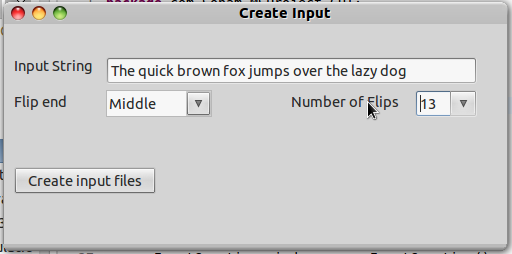
\includegraphics[width=5.2in]{inputcreationscreenshot.png}
  \end{center}
  \caption{Screen shot of GUI screen input, used to create the input files.}
  \label{fig:screenshotinputcreation}
\end{figure}

The click button on the GUI shown in figure 5.1 calls the createFile() function in class CreateInputFile, which 
is responsible for file creation. Details for both the class are shown in figure 5.2.

\begin{figure}
  \begin{center}
    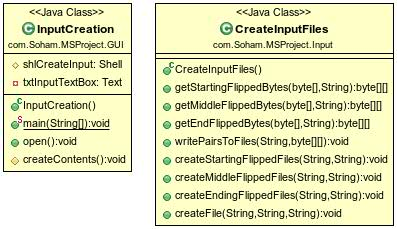
\includegraphics[width=4in]{Input.jpg}
  \end{center}
  \caption{Class diagram of the input creation.}
  \label{fig:UMLInputCreation}
\end{figure}

\subsection{Hash function implementation}

Each of the SHA-3 finalist hashing algorithm, were implemented in their own individual Java class. For the purpose
of the experiment, we only required the control over what input string went to the hashing algorithm, the number
of permutation rounds, and digest size in bits. Thus all the SHA-3 algorithms implement the interface "Hash" that
standardizes the call to each of finalist algorithm. The input string to the hash function, is the hexadecimal 
string representation of the ASCII bit value of the input string. The digest size is an integer from the following
four values 224, 256, 384 and 512. And the rounds can be anything between 1 and maximum number of rounds for a
given hash. For example in Keccak the number of rounds is 24, and if 25 is input in rounds, then the hashing will
be done for 24 rounds. So a safety check for a upward limit has not been built. By default, if you put zero, then
the recommended values of permutation rounds for the respective algorithm are used. The class diagram for the
SHA-3 hash function implementation is shown in figure 5.3.

\begin{figure}
  \begin{center}
    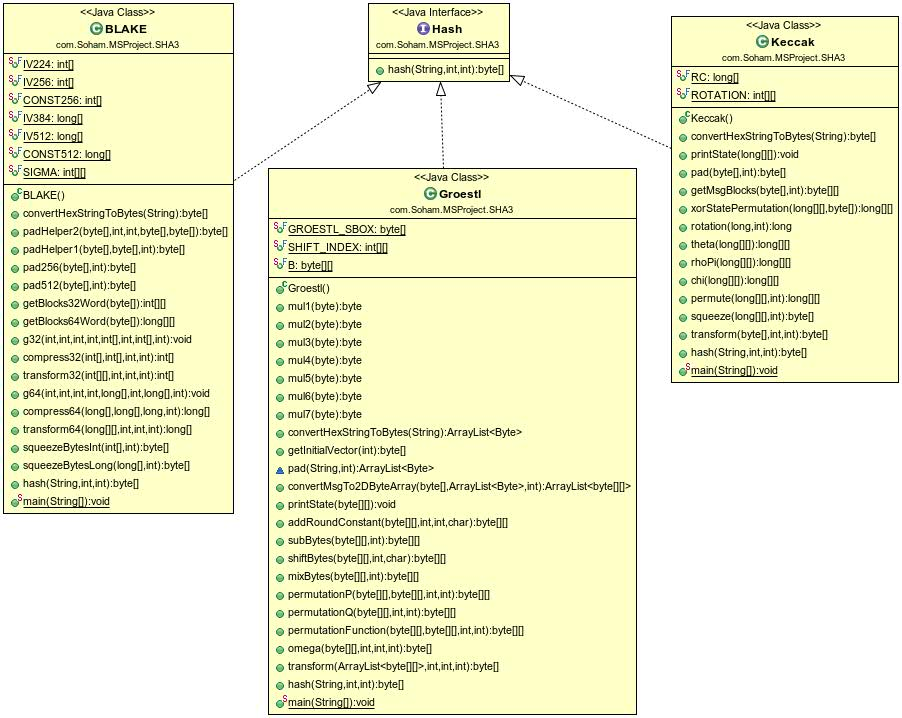
\includegraphics[width=6.8	in]{SHA3classes.jpg}
  \end{center}
  \caption{Class diagram of the classes for the 3 hash functions implemented.}
  \label{fig:UMLSHA3classes}
\end{figure}

\subsection{Experiment with different collision methods}

From the experiment selection dropdowns shown in figure 5.4, we can choose from the following factors
\begin{enumerate}
  \item The length of the chaining value that will be padded to the message, in bits.
  \item The algorithm for finding collision.
  \item The length of message digest in bits.
  \item The SHA-3 finalist algorithm, for hashing.
  \item Number of permuation rounds, for the hashing algorithm.
  \item The input case from start, middle or end, that you want to experiment with.
\end{enumerate}

\begin{figure}
  \begin{center}
    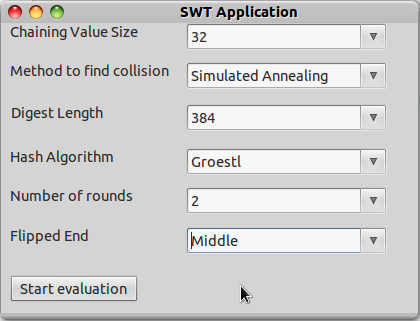
\includegraphics[width=4.25in]{experimentscreenshot.png}
  \end{center}
  \caption{Class diagram of the classes for the 3 hash functions implemented.}
  \label{fig:experimentscreenshot}
\end{figure}

The classes that instantiate the experiment, and their relation with the GUI class is shown in figure 5.5. It is 
the responsibility of the "Experiment" class, to go over the input files of the said category, and then provide 
the collision finding algorithms with the input message pairs, and instantiating them.

\begin{figure}
  \begin{center}
    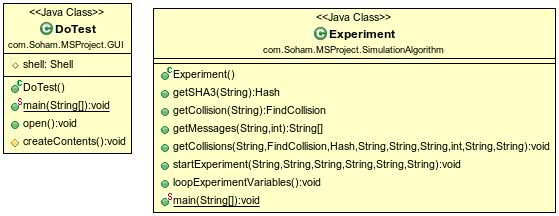
\includegraphics[width=5.65in]{ExperimentGUIClass.jpg}
  \end{center}
  \caption{Class diagram of the GUI class and the initiation of experiment.}
  \label{fig:UMLExperimentGUIClass}
\end{figure}

The Experiment class is the one that calls FindCollision algorithm, which is the parent class, that generates
the random chaining value as per the bit length provided. FindCollision evaluates the cost function, and generating
neighbourhood solution chaining values for the collision finding purpose. The relationship between the classes 
is shown in the UML class diagram shown in figure 5.6.

\begin{figure}
  \begin{center}
    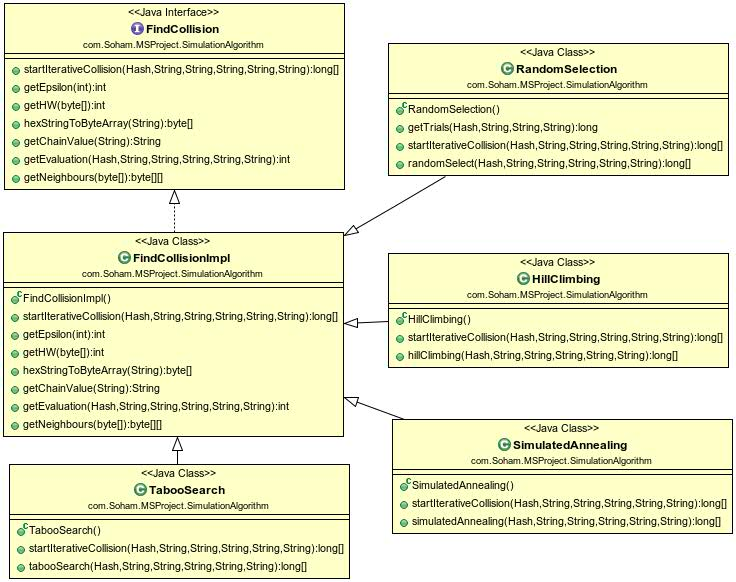
\includegraphics[width=7in]{FindCollisionClasses.jpg}
  \end{center}
  \caption{Class diagram of the classes for finding collisions.}
  \label{fig:UMLCollisionFindingClasses}
\end{figure}

\subsection{Testing the implemented code}

Code implementing hashing involves permuting and substituting large number of bits, resulting in subtle bugs that
can distort hash values. We have written, unit test cases to make sure, that our code works in individual case 
and as whole, so that the correctness of the results can be guaranteed with absence of bugs
or bias in the code. InputTest class is created to make sure, that the toggling of the bits is done as expected.
ExperimentTest class makes sure, that the correct parameters are called and passed like the correct hashing
algorithm, with the expected digest size and rounds etc. The SHA3Test class makes sure that the implementation of 
all the SHA-3 finalist create the right message digests as expected. Finally the test class HillClimbTest makes
sure that neighbourhood test for the chaining value is done properly. The class diagram for the test is shown in
figure 5.7.

\begin{figure}
  \begin{center}
    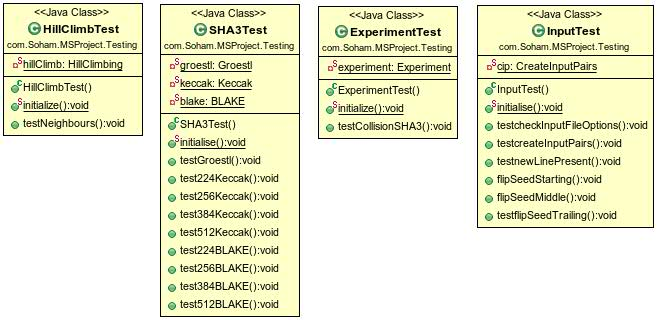
\includegraphics[width=6.75in]{testingcode.jpg}
  \end{center}
  \caption{Class diagram of the classes used for testing, using JUnit4.}
  \label{fig:UMLJUnitTestClasses}
\end{figure}
 % Research approach and methodology
%\chapter{Observations}

%% Obviously you need to delete these lines when you have written up your text

%\begin{itemize}
%\item{}  How did you analyze your hyptothesis? Experiments, what did you think were worth measuring, etc.
%\item{}  Based on your measurements and qualititative analyses, how well did your approach work out?
%\item{}  Use graphs, tables, and other diagrams to illustrate your analyses.
%\item{}  Based on your analyses, how well does your implementation or approach match your hypothesis?
%\item{}  What do you deduce from this effort? How would you change or tweak your hypothesis? 

%\end{itemize}

For the time being, here is my hypothesis, or the premise of my question. Keccak has been selected over BLAKE and
Groestl for what? Is there is a basis that Keccak's property is still comparitively immune to zero sum distinguisher
compared to BLAKE and Groestl in the reduced versions. This is what, I would like to find out and examine.
       % Put the observation table, and the figures.
\chapter{Conclusions and future work}

\section{Validity of the hypothesis}

In section 4.4 two hypothesis were suggested, both have been sort of some what disproved. When the reduced version
of an algorithm is only done by reducing the number of rounds, then for just rounds 1 and 2, Keccak performs worse
than BLAKE and Gr{\o}stl. Also from the numbers and taking into account the number of success in getting collisions,
hill climbing performs better than simulated annealing and tabu search. Random selection also performs, some what 
comparable to simulated annealing, but not much. Suggesting that for reduced rounds, that random selection could
also be used to find near collisions.

\subsection{Collision resistance of SHA-3 finalist in reduced rounds}

For 1 round permutation, all the algorithms should almost equivalent weakness, that is collision in almost all instances
that is message pairs, and trial. However for Keccak for the three collision finding algorithms hill climbing, simulated
annealing, and random selection; collisions were seen in every instance and trial. This behaviour is again noticed
in Keccak for permuation of round 2; however for BLAKE and Gr{\o}stl, this number of trials and instances in which
collision could be found are reduced.

However as the permutation rounds are increased to 3 and 4, the resistance to collision finding algorithms for Keccak
becomes equivalent to that of BLAKE and Gr{\o}stl. For digest sizes, of 224 and 256; some message pairs do show
collision in trials less than 10. But for digest sizes of 384 and 512; no collisions are found.

\subsection{Feasibility of the collision algorithms}

From the collision algorithms; hill climbing seems to be the most optimised in terms of collision finding to time required
ratio. Tabu search performs the worst, in terms of collision to CPU time required. For example using tabu search on 
Gr{\o}stl for message digest of 224 bits, and rounds 1 and 2; tabu search required around 334894 iterations on average,
without any collisions. For the same conditions hill climbing did not require more than 900 iterations, with some success.

At lower permutation rounds like 1 and 2, for Keccak; and for round 1 for BLAKE and Gr{\o}stl random selection is as 
effective as hill climbing and simulated annealing. Even for higher rounds like 3 and 4; for lower digest sizes of 224
and 256, random selection was able to find collision amongst all three SHA-3 candidate algorithms in around 10 instances 
in trials less than 10. This performance is comparable to that of simulated annealing.

Tabu search performs poorly, given that it goes for the steepest descent approach. Tabu search tries to pick the best 
chaining value from the neighbourhood, where the k-bit neighbourhood, whose size is roughly equal to $n^{2}$ where n
is the bit length of the chaining value. Also the tabu search has to go through elements of neighbourhood comparing each
of them with the tabu list, before inserting them into the candidate set where they will be considered as solution.
This places additional overhead on the algorithm performance. The tabu list can be made up of states, solutions previously
found, moves previously made. For our case the best element for tabu list would have been elements from previous iteration
that were not selected, but this still makes our set large. Although the process can be speed up, by getting the best
element from neighbourhood during neighbourhood creation, but you still have the over head of comparing the elements
twice for the best element and the comparing with tabu list. The problem does not mould well, with the tabu search
solution, because trying to store state, previous solution, or moves in tabu list are all expensive.

Simulated annealing though trying to avoid the local minima, does not perform any better than hill climbing, when finding
near collisions. Over trials over 256 and 128, and chaining values 32 and 64; simulated annealing found far fewer collisions
than hill climbing. While hill climbing was able to find collision in instances in more than 50\% of the message
pairs for each of the SHA-3 algorithm for message digest of 224 and 256, for permutation rounds of 3 and 4. But 
simulated annealing is only able to find collision in 1 instance out of 60 for 1 trial.

\section{Effect of digest size}

It seems as the digest size is increased, the near collision resistance increases, only if the rounds are above 2. The
input text here "The quick brown fox jumps over the lazy dog" was of 344 bits, and as per table 7.1 even with 32 bit
chaining value, the entire message is treated in one part itself, as seen from table 7.1. Thus our modifications to 
the message pairs do make it through in one go, rather than blocks of message from the pairs which have all bits same.

The reason higher message digests seem to have more collision resistance may be due to the fact that they have more
bits to shuffle around, thus making it harder for simple algorithms without any heuristics to find the collisions. Note
should be made that near collisions in this case is done when bits matching are more than 65\% of the digest length.
So it could be that bits upto 64\% might match and yet be rejected not as near collision found. Also the higher
digest sizes like 384 and 512 only show collision resistance only if applied with rounds 3 and 4.

Thus the minimum security recommendation for collision avoidance would be go for digest sizes of 384 and above.

\begin{table}
  \begin{center}
    \begin{tabular}{ *{5}{| c |} }                                 \hline
     \multirow{2}{*}{Hash algorithm} & \multicolumn{4}{|c|}{Digest size} \\ \cline{2-5}
               & 224  & 256  & 384  & 512  \\ \hline
     BLAKE     & 512  & 512  & 1024 & 1024 \\ \hline
     Gr{\o}stl & 512  & 512  & 1024 & 1024 \\ \hline
     Keccak    & 1152 & 1088 & 832  & 576  \\ \hline
    \end{tabular}
    \caption{Number of input bits to one function block, in the respective SHA-3 finalist algorithm}
  \end{center}
\end{table}

\begin{table}
  \begin{center}
    \begin{tabular}{ *{5}{| c |} }                                 \hline
     \multirow{2}{*}{Hash algorithm} & \multicolumn{4}{|c|}{Digest size} \\ \cline{2-5}
               & 224 & 256 & 384 & 512 \\ \hline
     BLAKE     & 14  & 14  & 16  & 16  \\ \hline
     Gr{\o}stl & 10  & 10  & 14  & 14  \\ \hline
     Keccak    & 24  & 24  & 24  & 24  \\ \hline
    \end{tabular}
    \caption{Number of permutation rounds, in the respective SHA-3 finalist algorithm}
  \end{center}
\end{table}

\section{Effects of the number of rounds}

From the observation of tables 6.7 to 6.20, we can conclude that higher the number of permutation rounds, the
more is the collision resistance. Rounds 1 and 2, can be considered as not secure. It should be noted that
for permutation rounds 1 and 2; Keccak seems to perform poorly against BLAKE and Gr{\o}stl. But as rounds
are increased to 3 and 4, the performance of Keccak with respect to other algorithms is comparable. 

On the basis of observation it can be stated that, at minimum 3 rounds of permutation are required, and 4 to 
be secure as per the results of this experiment with limited resources. Please note that as per table 7.2,
the recommended number of permutation rounds for each SHA-3 finalist algorithm is different. While Gr{\o}stl
has the least number of rounds, Keccak has most number of rounds. This could be one explanation of Gr{\o}stl
and BLAKE's, better performance though not most ideal; than Keccak for rounds 1 and 2.

\section{Chaining value length}

Longer chaining value do not seem to help in getting near collisions. For perfect collisions, longer chaining values
might be helpful. However for near collisions, shorter chaining values work fine. With larger chaining values,
the number of times the algorithm has to loop through also increases. For increase in chaining value from 32 bits
to 64 bits, the loop execution increased by factor of 3 times more than what it required for 32 bits.

\section{Bit differences in message in particular positions}

All the SHA-3 algorithms displayed lack of diffusion property if any, irrespective of input bit updated in any
of the three positions start, middle and end specified in the message input string. The bit update made to middle,
and end to the input message are almost equivalent, since, the input message is padded with the chaining value. 
Thus we do not experiment with the bits updated at the end of the input string, only with bits updated at start
of the string or in the middle of the string. Since in the experiment trials the chaining value is chosen randomly,
hence small differences in finding collisions amongst the input, for a given hashing algorithm, digest size and round
can be ignored. Based on this fact, it seems that diffusion in the given algorithm is place agnostic. 

\section{Future work}

\begin{enumerate}
\item This experiment can be repeated with the two other finalist algorithm Skein and JH, alongwith Keccak.
\item Instead of reducing the number of rounds, the reduced version of the finalist algorithm could be obtained
by reducing the state size, and repeating this experiment.
\item Experiments can also be done with other combinations of factors of hashing algorithms, like reducing the
digest size, but increasing the number of rounds.
\item In this experiment, the near collision was benchmarked at 65\% of the output bits match. Instead further work
can be done to find the effort required to find perfect collisions for message pairs for reduced rounds for
certain hashing algorithms.
\end{enumerate}
    % Evaluations and expected outcomes and future work

%%%%%%%%%%%%%%%%%%%%%%%%%%%%%%%%%%%%%%%%%%%%%%%%%%%%%%%%%%%%%%%%%%%%%%%%%%%%%%%

%%%%%%%%%%%%%%%%%%%%%%%%%%%%%%%%%%%%%%%%%%%%%%%%%%%%%%%%%%%%%%%%%%%%%%%%%%%%%%%
\bibliographystyle{plain}
% Single space the bibliography to save space.
\begin{singlespace}
\bibliography{CapstoneBib}
\end{singlespace}
%%%%%%%%%%%%%%%%%%%%%%%%%%%%%%%%%%%%%%%%%%%%%%%%%%%%%%%%%%%%%%%%%%%%%%%%%%%%%%%

%%%%%%%%%%%%%%%%%%%%%%%%%%%%%%%%%%%%%%%%%%%%%%%%%%%%%%%%%%%%%%%%%%%%%%%%%%%%%%%
% The appendices are (of course) optional.
\appendix
\chapter{Miscellaneous Proofs, Theorems and Figures}

\begin{enumerate}
\item Following is the S-box used in Gr{\o}stl. For an input x, you do a logical AND of x with 
  f0 and with 0f. The first value obtained is used for column location and second for row location.
  The row and column location is used to identify the cell that will be used for substitution.
  \begin{table}[h]
  \begin{center}
    \begin{tabular}{ c |  *{16}{c}}
       & 00 & 01 & 02 & 03 & 04 & 05 & 06 & 07 & 08 & 09 & 0a & 0b & 0c & 0d & 0e & 0f \\ \hline
    00 & 63 & 7c & 77 & 7b & f2 & 6b & 6f & c5 & 30 & 01 & 67 & 2b & fe & d7 & ab & 76 \\ 
    10 & ca & 82 & c9 & 7d & fa & 59 & 47 & f0 & ad & d4 & a2 & af & 9c & a4 & 72 & c0 \\
    20 & b7 & fd & 93 & 26 & 36 & 3f & f7 & cc & 34 & a5 & e5 & f1 & 71 & d8 & 31 & 15 \\
    30 & 04 & c7 & 23 & c3 & 18 & 96 & 05 & 9a & 07 & 12 & 80 & e2 & eb & 27 & b2 & 75 \\
    40 & 09 & 83 & 2c & 1a & 1b & 6e & 5a & a0 & 52 & 3b & d6 & b3 & 29 & e3 & 2f & 84 \\
    50 & 53 & d1 & 00 & ed & 20 & fc & b1 & 5b & 6a & cb & be & 39 & 4a & 4c & 58 & cf \\
    60 & d0 & ef & aa & fb & 43 & 4d & 33 & 85 & 45 & f9 & 02 & 7f & 50 & 3c & 9f & a8 \\
    70 & 51 & a3 & 40 & 8f & 92 & 9d & 38 & f5 & bc & b6 & da & 21 & 10 & ff & f3 & d2 \\
    80 & cd & 0c & 13 & ec & 5f & 97 & 44 & 17 & c4 & a7 & 7e & 3d & 64 & 5d & 19 & 73 \\
    90 & 60 & 81 & 4f & dc & 22 & 2a & 90 & 88 & 46 & ee & b8 & 14 & de & 5e & 0b & db \\
    a0 & e0 & 32 & 3a & 0a & 49 & 06 & 24 & 5c & c2 & d3 & ac & 62 & 91 & 95 & e4 & 79 \\
    b0 & e7 & c8 & 37 & 6d & 8d & d5 & 4e & a9 & 6c & 56 & f4 & ea & 65 & 7a & ae & 08 \\
    c0 & ba & 78 & 25 & 2e & 1c & a6 & b4 & c6 & e8 & dd & 74 & 1f & 4b & bd & 8b & 8a \\
    d0 & 70 & 3e & b5 & 66 & 48 & 03 & f6 & 0e & 61 & 35 & 57 & b9 & 86 & c1 & 1d & 9e \\
    e0 & e1 & f8 & 98 & 11 & 69 & d9 & 8e & 94 & 9b & 1e & 87 & e9 & ce & 55 & 28 & df \\
    f0 & 8c & a1 & 89 & 0d & bf & e6 & 42 & 68 & 41 & 99 & 2d & 0f & b0 & 54 & bb & 16 \\
    \end{tabular}
  \end{center}
  \end{table}

  \item
 $ B = \begin{bmatrix}
    02 & 02 & 03 & 04 & 05 & 03 & 05 & 07 \\
    07 & 02 & 02 & 03 & 04 & 05 & 03 & 05 \\
    05 & 07 & 02 & 02 & 03 & 04 & 05 & 03 \\
    03 & 05 & 07 & 02 & 02 & 03 & 04 & 05 \\
    05 & 03 & 05 & 07 & 02 & 02 & 03 & 04 \\
    04 & 05 & 03 & 05 & 07 & 02 & 02 & 03 \\
    03 & 04 & 05 & 03 & 05 & 07 & 02 & 02 \\
    02 & 03 & 04 & 05 & 03 & 05 & 07 & 02 \\
  \end{bmatrix}$

\end{enumerate}

%\chapter{Code Listing}

This is an optional appendix and can be eliminated if you don't have anything 
to share here.


%\chapter{User Manual}

This is an optional appendix and can be eliminated if you don't have anything 
to share here.


% ...
%%%%%%%%%%%%%%%%%%%%%%%%%%%%%%%%%%%%%%%%%%%%%%%%%%%%%%%%%%%%%%%%%%%%%%%%%%%%%%%
\end{document}
